\chapter{Metodolog\'ia}
La investigaci\'on se trabaj\'o con un enfoque mixto debido que integra dos m\'etodos:
\begin{itemize}
	\item \textbf{Cualitativo:} Dentro de la investigaci\'on se utiliz\'o el m\'etodo de observaci\'on para seleccionar el movimiento de an\'alisis por cada equipo deportivo, as\'i mismo el investigador realiz\'o grupos focales con los entrenadores y atletas de cada equipo deportivo, con la finalidad de documentar los pasos correctos para realizar un movimiento v\'alido.
	\item \textbf{Cuantitativo:} En este proyecto de ingenier\'ia se utiliz\'o el Kinect para grabar v\'ideos de atletas realizando el movimiento v\'alido, posteriormente por cada v\'ideo se etiquet\'o los fotogramas con un valor decimal, seguidamente se utiliza estos valores para entrenar el algoritmo Random Forest Regression, con la finalidad de detectar los pasos de un movimiento v\'alido. Por otra parte, se cre\'o un algoritmo clasificador que clasifica si un movimiento es v\'alido o inv\'alido a partir de la detecci\'on de los pasos.
\end{itemize}
\section{Sujetos}
El departamento de deportes de la Universidad Rafael Land\'ivar, le proporcion\'o al investigador, la colaboraci\'on de todos los deportes -e.g. F\'utbol, voleibol, baloncesto, tenis, banda, zumba, atletismo, nataci\'on, taekwondo, tenis de mesa y animaci\'on-. Lo cual el investigador tuvo que realizar filtros para seleccionar la poblaci\'on, descartando aquellos deportes que entrenaban en las federaciones nacionales de Guatemala -i.e. Lugares externos a la Universidad Rafael Land\'ivar-, entre ellos estaban: Atletismo, nataci\'on y tenis. Por otro lado, el investigador apart\'o los deportes que se ejercitaban dentro de una cancha deportiva debido a la dificultad de colocar todos los materiales necesarios del proyecto para la toma de datos, por lo cual se elimin\'o los deportes de:  f\'utbol, voleibol y baloncesto. Finalmente, el investigador ignor\'o los deportes de banda y zumba, ya que son actividades que se trabajan en conjunto con otros departamentos de la Universidad Rafael Landivar -e.g. Unidad de artes Land\'ivar-. De modo que el investigador seleccion\'o los siguientes deportes:
\begin{itemize}
	\item \textbf{Tenis de mesa:} Deporte de raqueta que se juega sobre una mesa rectangular de manera individual o en parejas, con el fin objetivo de golpear una peque\~na pelota.
	\item \textbf{Animaci\'on:} Deporte grupal que combina la m\'usica y gimnasia, a partir de rutinas de baile que entusiasma un p\'ublico o evento deportivo.
	\item \textbf{Taekwondo:} Deporte individual basado en el arte marcial coreano moderno, que consiste en el uso de los pies, brazos y pu\~nos dentro de un combate.
\end{itemize}
\subsection{Primer tipo} \label{sj:1t}
Define la cantidad de sujetos que participaron en la colecta de los datos para la creaci\'on del modelo de reconocimiento del movimiento, a partir de tres fases distintas:
\begin{itemize}
	\item \textbf{Construcci\'on:} Atletas que construyeron el modelo continuo de la m\'aquina de aprendizaje.
	\item \textbf{Pruebas:} Muestra de usuarios que se emple\'o para el c\'alculo de los m\'argenes de  errores del pron\'ostico del modelo.
	\item \textbf{Validaci\'on:} Conjunto de deportistas que realizaron las pruebas al modelo en tiempo real.
\end{itemize}
\subsubsection{Equipo de animaci\'on de la Universidad Rafael Land\'ivar} \label{sj:1t:ani}
\begin{table}[H]
\begin{center}
\caption{Muestra del equipo de animadoras}
\label{tab:MuestraCheerleaders}
\begin{tabular}{lc}
\hline
\multicolumn{1}{|l|}{\textbf{Descripci\'on}} & \multicolumn{1}{l|}{\textbf{Cantidad}} \\ \hline
\multicolumn{1}{|l|}{Atletas para la construcci\'on del modelo} & \multicolumn{1}{c|}{6} \\ \hline
\multicolumn{1}{|l|}{Atletas para las pruebas del modelo} & \multicolumn{1}{c|}{1} \\ \hline
\multicolumn{1}{|l|}{Atletas para la validaci\'on del modelo} & \multicolumn{1}{c|}{2} \\ \hline
\multicolumn{1}{|r|}{Total de atletas} & \multicolumn{1}{c|}{9} \\ \hline
\textbf{Fuente:} Observaci\'on del investigador durante el trabajo de campo.
\end{tabular}
\end{center}
\end{table}
\subsubsection{Equipo de tenis de mesa de la Universidad Rafael Land\'ivar}\label{sj:1t:ten}
\begin{table}[H]
\begin{center}
\caption{Muestra del equipo de tenis de mesa}
\label{tab:MuestraTenis}
\begin{tabular}{lc}
\hline
\multicolumn{1}{|l|}{\textbf{Descripci\'on}} & \multicolumn{1}{l|}{\textbf{Cantidad}} \\ \hline
\multicolumn{1}{|l|}{Atletas para la construcci\'on del modelo} & \multicolumn{1}{c|}{5} \\ \hline
\multicolumn{1}{|l|}{Atletas para las pruebas del modelo} & \multicolumn{1}{c|}{1} \\ \hline
\multicolumn{1}{|l|}{Atletas para la validaci\'on del modelo} & \multicolumn{1}{c|}{3} \\ \hline
\multicolumn{1}{|r|}{Total de atletas} & \multicolumn{1}{c|}{9} \\ \hline
\textbf{Fuente:} Observaci\'on del investigador durante el trabajo de campo.
\end{tabular}
\end{center}
\end{table}
\subsubsection{Equipo de taekwondo de la Universidad Rafael Land\'ivar}\label{sj:1t:tae}
\begin{table}[H]
\begin{center}
\caption{Muestra del equipo de taekwondo}
\label{tab:MuestraTaekwondo}
\begin{tabular}{lc}
\hline
\multicolumn{1}{|l|}{\textbf{Descripci\'on}} & \multicolumn{1}{l|}{\textbf{Cantidad}} \\ \hline
\multicolumn{1}{|l|}{Atletas para la construcci\'on del modelo} & \multicolumn{1}{c|}{13} \\ \hline
\multicolumn{1}{|l|}{Atletas para las pruebas del modelo} & \multicolumn{1}{c|}{1} \\ \hline
\multicolumn{1}{|r|}{Total de atletas} & \multicolumn{1}{c|}{14} \\ \hline
\textbf{Fuente:} Observaci\'on del investigador durante el trabajo de campo.
\end{tabular}
\end{center}
\end{table}
\subsection{Segundo tipo} \label{sj:2t}
A continuaci\'on se muestra un organigrama de la estructura del departamento de deportes de la Universidad Rafael Land\'ivar, en ella se muestra todos los profesionales que aportaron en la investigaci\'on:
\begin{figure}[H]
	\caption{Organigrama del departamento de deportes de la Universidad Rafael Land\'ivar}
	\label{fig:orgDeportes}
	\centering
	\includegraphics[width=450px,height=170px]{graphics/orgDeportes.png} \\
	\textbf{Fuente:} Elaborado por el autor de tesis
\end{figure}
\subsection{Unidades de an\'alisis} \label{sj:ua}
Para el presente proyecto se utiliz\'o como referencia el manual de acondicionamiento de fuerza y prevenci\'on de lesiones  \cite{arbour2006strength}, la cual describe los movimientos ideales para el calentamiento  y estiramiento de una rutina. (Ver secci\'on de anexos \ref{anx:warmup}).
\section{Instrumentos}\label{ins}
El conjunto de instrumentos se elabor\'o con los  siguientes recursos:
\begin{itemize}
\item Humanos
	\begin{itemize}
	\item Profesionales -i.e. Entrenadores-.
	\item Atletas
	\item Investigador
	\end{itemize}
\item No humanos
	\begin{itemize}
	\item Mesa de soporte con una altura de 0.70 metros.
	\item Cable de extensi\'on el\'ectrico de 2.00 metros. 
	\item Computadora port\'atil
		\begin{itemize}
		\item Conector de carga de alimentaci\'on
		\end{itemize}
	\item Sensor Kinect
		\begin{itemize}
		\item Adaptador del Kinect
		\end{itemize}
	\end{itemize}
\end{itemize}
\subsection{Formulario de registro de movimiento} \label{ins:frmMov}
Este formulario se adjunta en anexos (ver figura \ref{fig:frmWhiteMov}), la cual tiene como objetivo describir el movimiento de cada equipo deportivo. Por otra parte, el formulario est\'a compuesto por los siguientes incisos:
\begin{itemize}
	\item \textbf{Nombre del movimiento:} Nombre que se identifica en gu\'ias deportivas o de salud.
	\item \textbf{Descripci\'on del movimiento: } Contesta la pregunta: ?`Qu\'e es el movimiento?
	\item \textbf{Movimiento unilateral:} Si es afirmativo, el movimiento trabaja con solo una parte del cuerpo (izquierda o derecha, ejemplo una patada), en caso contrario, se considera todas las partes del cuerpo (izquierda y derecha, ejemplo un salto).
	\item \textbf{Partes del cuerpo ignorada:} M\'ultiples respuestas que identifican las articulaciones ignoradas -i.e. Debido que no es informaci\'on relevante para el movimiento-:
	\begin{itemize}
		\item \textbf{Brazo derecho o izquierdo:} Ignora las siguientes articulaciones (seg\'un su lado): Pulgar, dedo del medio, mano, codo, hombro, centro de los hombros, cuello, cabeza y espalda.
		\item \textbf{Cuerpo inferior:} Ignora las siguientes articulaciones (en ambos lados): Centro de cadera, caderas, rodillas, tobillos y pies.
	\end{itemize}
		\item \textbf{N\'umero de pasos:} Cantidad de pasos del movimiento.
		\item \textbf{Offset del paso:} Valor que separa las etiquetas por partes iguales.
		\item \textbf{Valor de identificaci\'on:} Valor que reconoce las etiquetas por partes iguales.
		\item \textbf{Detalle por paso:} Es  importante conocer:
			\begin{itemize}
		\item \textbf{Paso:} N\'umero \'unico que identifica el paso.
		\item \textbf{Diagrama:} Imagen visual del paso -i.e. Seguimiento del esqueleto-.
		\item \textbf{Descripci\'on del paso:} Responde la pregunta: ?`Cu\'al es la postura del cuerpo durante ese paso?
		\item \textbf{Etiqueta:} N\'umero \'unico que identifica el paso a partir de la probabilidad de movimiento.
	\item \textbf{Rango de identificaci\'on:} Rango m\'aximo que identifica el paso dentro de la probabilidad del movimiento.
	\end{itemize}
\end{itemize}
\subsection{Formulario de registro de rutina} \label{ins:frmRout}
Formulario adjuntado en anexos (Ver figura \ref{fig:frmWhiteRout}), tiene como funci\'on identificar los ejercicios de calentamiento  previamente a realizar el movimiento seleccionado por cada equipo deportivo, adem\'as de estandarizar el n\'umero de repeticiones del movimiento por cada atleta, a partir de los siguientes puntos:
\begin{itemize}
	\item \textbf{Descripci\'on del calentamiento:} Detalla el tipo de calentamiento -e.g. Calentamiento con tu propio peso, calentamiento dentro de un ambiente, calentamiento a partir de objetos-.
	\item \textbf{Movimientos:} Lista los movimientos que se realizan durante el calentamiento (Validado por el formulario de registro de movimiento).
	\item \textbf{Series:} Cantidad de veces que debe realizar un atleta, un conjunto de repeticiones del movimiento.
	\item \textbf{Repeticiones:} Cantidad de repeticiones del movimiento.
	\item \textbf{Tiempo:} Duraci\'on del calentamiento.
	\item \textbf{Im\'agenes:} Fotograf\'ias tomadas durante el entrenamiento de cada equipo deportivo.
	\item \textbf{Nombre del movimiento:} Movimiento seleccionado por cada equipo deportivo  (validado por el formulario de registro de movimiento).
	\item \textbf{Rutina:} Describe el tipo de rutina para la captura de datos:
	\begin{itemize}
		\item \textbf{For time:} M\'axima cantidad de repeticiones del movimiento, durante un tiempo establecido.
		\item \textbf{Escaleras:} N\'umeros de repeticiones establecidas, separadas por series.
	\end{itemize}	
\end{itemize}
\subsection{Interfaces de usuarios} \label{ins:UI}
Aplicaciones que interact\'uan con el usuario para la recolecci\'on de datos, en donde se trabajan con  tres tipos:
\subsubsection{Windows presentation foundation (WPF)}
\label{ins:UI:wpf}
El desarrollador, \citeA{wpf2019}, menciona que este tipo de interfaz permite crear aplicaciones de escritorio con la tecnolog\'ia .NET, la cual es soportado desde windows XP hasta la \'ultima versi\'on de windows -i.e. windows 10-. Por lo tanto, en el presente proyecto se utiliz\'o este tipo de interfaz para la construcci\'on del seguimiento del esqueleto, generado por los siguientes kits de desarrollo de software:
\begin{itemize}
	\item \textbf{Windows inputs:} Herramienta que permite crear elementos de un formulario -e.g. Botones, cajas de textos- \cite{wpfWindows2019}.
	\item \textbf{Windows media:} Herramientas que permiten renderizar el seguimiento del esqueleto en tiempo real a partir de pinceles, colores, formas y dibujos \cite{WindowMedia2019}.
	\item \textbf{Windows threading:} Herramientas que permiten crear temporizadores para la renderizaci\'on del seguimiento del esqueleto en un per\'iodo del tiempo (30 fotogramas por segundos) \cite{WindowThreading2019}.
	\item \textbf{Kinect:} Herramientas que permiten acceder a las funcionalidades del sensor \cite{WindowKinect2019}, tales:
	\begin{itemize}
					\item \textbf{Body frame reader:} Obtiene la informaci\'on del seguimiento del esqueleto.
				\item \textbf{Estado del sensor:} Activo, pausa, no detectado e inactivo.
				\item \textbf{Datos del Visual Gesture Builder:} Normalizaci\'on de datos del sensor del Kinect para el uso del modelo de reconocimiento de movimiento.
			\item \textbf{Joint type:} Enumeradores que listan las articulaciones del seguimiento del esqueleto -e.g. Manos, codos, hombros-.
			\item \textbf{Visualizaci\'on de los recursos de los fotogramas para Visual Gesture Builder:} Interpreta la base de datos de gesturas y posiciones de un movimiento.
	\end{itemize}	 
\end{itemize}
A partir de los kits de desarrollo se crearon 2 aplicaciones para la captura de informaci\'on.
\paragraph{Detecci\'on de profundidad}\mbox{} \\ \label{ins:UI:wpf:depth}
Esta aplicaci\'on tiene como objetivo recolectar la distancia correcta de profundidad entre el atleta y el Kinect, tomando en cuenta una articulaci\'on de an\'alisis, adem\'as de la altura del usuario medida desde la cabeza hasta los pies, tal como se presenta en la imagen de la interfaz gr\'afica de detecci\'on de profundidad:
\begin{figure}[H]
	\caption{Interfaz gr\'afica de detecci\'on de profundidad entre el usuario y el sensor}
	\label{fig:appDepth}
	\centering
	\includegraphics[width=380px,height=200px]{graphics/appProfundidad.png} \\
	\textbf{Fuente:} Aplicaci\'on elaborada por el autor de tesis
\end{figure}
Esta interfaz se compone por 5 componentes:
\begin{enumerate}[A.]
    \item Selecci\'on de una articulaci\'on de an\'alisis.
    \item Bot\'on que empieza las funcionalidades del seguimiento del esqueleto.
    \item Bot\'on que finaliza las funcionalidades del seguimiento del esqueleto.
    \item Conjunto de paneles de controles que muestran una imagen en tiempo real del seguimiento del esqueleto, adem\'as de la altura (en metros) del usuario y la distancia de profundidad (en metros) entre el atleta y el sensor.
        \item Bot\'on que permite copiar a una hoja de observaci\'on (ver anexos, cuadro \ref{tab:obsDepth}) los siguientes datos respectivos: N\'umero de identificaci\'on de la articulaci\'on, la distancia de profundidad y la altura del usuario.
\end{enumerate}
\paragraph{Evaluaci\'on del movimiento}\mbox{} \\\label{ins:UI:wpf:evaluate}
Aplicaci\'on realizada por el autor del usuario, cuya funcionalidad es programar una rutina de tabata a partir del movimiento de cada equipo deportivo, mostrado en la interfaz gr\'afica de evaluaci\'on de un movimiento:
\begin{figure}[H]
	\caption{Interfaz gr\'afica de evaluaci\'on de un movimiento}
	\label{fig:appEvaluate}
	\centering
	\includegraphics[width=380px,height=250px]{graphics/appEvaluacion.png} \\
	\textbf{Fuente:} Aplicaci\'on elaborada por el autor de tesis
\end{figure}
Dicha interfaz se divide en 13 componentes:
\begin{enumerate}[A.]
    \item Bot\'on que permite seleccionar el archivo de base de datos del reconocimiento del movimiento.
    \item Bot\'on que permite seleccionar el archivo json que contiene toda la informaci\'on respectiva del movimiento (ver anexos, c\'odigo  \ref{code:jsonMeta}).
    \item Bot\'on que permite seleccionar la direcci\'on del archivo de resultado de tabata.
    \item Bot\'on que permite activar todas las funcionalidades del Kinect.    
    \item Bot\'on que permite detener todas las funcionalidades del Kinect. 
    \item Bot\'on que permite comenzar la rutina de tabata (en tiempo real).
   \item  Caja de texto num\'erica que indica la cantidad de tiempos de trabajos y descansos del atleta durante su rutina de tabata.
   \item  Caja de texto num\'erica que se\~nala el tiempo de descanso durante una rutina.
   \item  Caja de texto n\'umerica que muestra el tiempo de trabajo durante una rutina -i.e. Durante este tiempo, el atleta debe realizar la cantidad m\'axima de repeticiones-.
   \item  Etiqueta de articulaci\'on de an\'alisis para medir la distancia de profundidad entre el atleta y el sensor.
   \item  Etiqueta de la altura  recomendada (en metros)  del sensor y el suelo.
      \item  Etiqueta de la distancia m\'inima y m\'axima de profundidad del atleta con respecto al sensor, y por otra parte indica la distancia profundidad actual del usuario y el sensor.
      \item Conjunto de paneles de controles que muestran:
      \begin{itemize}
            \item  El seguimiento del esqueleto en tiempo real.
            \item  Estado actual de la rutina: Inicio, trabajo, descanso y fin.
            \item  Temporizador de cuenta regresiva del tiempo de trabajo o descanso (en segundos).
             \item  Serie actual que est\'a trabajando el atleta.
             \item  Contador de repeticiones de la serie actual.
              \item \'Ultimo paso ejecutado por el atleta (comenzando desde 0).   
             \item  Valor de probabilidad del movimiento -i.e. Factor del movimiento-.
             \item  Temporizador que mide el tiempo    empleado en la rutina (en segundos).
      \end{itemize}
\end{enumerate}
Ya definido los componentes de la interfaz, se debe tomar en cuenta que al finalizar cada rutina tabata  el programa genera un archivo json (ver anexos, c\'odigo  \ref{code:tabata}), con los siguientes resultados:
\begin{itemize}
	\item \textbf{Analizador de variables:} Indica las variables que fueron configurado en un tabata: Tiempo de descanso, tiempo de trabajo y la cantidad de series.
	\item  \textbf{Resultados generales:} Muestran los resultados del volumen de repeticiones  y el tiempo total empleado en la rutina de tabata.
	\item  \textbf{Resistencia:} Vector de informaci\'on que permite construir la gr\'afica de la rutina tabata, a partir de los siguientes par\'ametros:
	   \begin{itemize}  
   	\item \textbf{Uid:} C\'odigo \'unico de identificaci\'on de la gr\'afica.
   	\item \textbf{Label:} Nombre de la gr\'afica.
   	\item \textbf{ShowLine:} Condici\'on que permite dibujar la l\'inea de la tendencia de la gr\'afica.
    \item \textbf{Data:} Vector de datos que conforma la gr\'afica, en donde los datos del eje x, representan el tiempo de rutina (en segundos), y los datos del eje y, significan las repeticiones acumulada durante ese tiempo de rutina.
   \end{itemize}     
    \item \textbf{Potencia:} Cantidad de repeticiones m\'axima del movimiento, en el menor tiempo posible.
    \item \textbf{Velocidad:} Se divide en dos resultados:
           \begin{itemize}
       \item Cantidad promedio de repeticiones en una serie.
       \item Tiempo promedio por una repetici\'on
       \end{itemize}
\end{itemize} 
\subsubsection{Web}\mbox{} \\
\label{ins:UI:web}
Interfaz de usuario que permite capturar la informaci\'on de los formularios de movimiento, a partir de la siguiente arquitectura:
\begin{figure}[H]
	\caption{Arquitectura web}
	\label{fig:architectureWeb}
	\centering
	\includegraphics[width=430px,height=220px]{graphics/webArchitecture.PNG} \\
	\textbf{Fuente:} Elaborado por el autor de tesis
\end{figure}
\begin{itemize}
\item Frontend
	\begin{itemize}
	\item \textbf{Web}: Interfaz agradable para el usuario, cuya finalidad es realizar llamadas a las aplicaciones de negocio y servidor de archivos.
	\end{itemize}
\item Backend
	\begin{itemize}
	\item \textbf{Business api:} Maneja todas las  funciones l\'ogicas del giro de negocios -e.g. Insertar movimiento, leer movimiento, resultados de rutina-.
	\item \textbf{File sistem:} Interfaz de programaci\'on de aplicaciones que se encarga de almacenar los archivos de metadata que define una base de datos del movimiento.
		\item \textbf{Linux files:} Servidor encargado de almacenar los archivos de bases de datos del movimiento.
		\item \textbf{Mongo DB:} Servidor de bases de datos no relacional, que se encarga de almacenar informaci\'on respectiva del movimiento.
	\end{itemize}
\item Entornos de trabajo
\begin{itemize}
\item \textbf{Angular 7:} Herramienta que facilita la creaci\'on y el mantenimiento de una aplicaci\'on web \cite{angular2019}.
\item \textbf{Argon dashboard angular:} Herramienta  que facilita realizar una aplicaci\'on responsiva -i.e. Adaptable a cualquier dispositivo a partir de un navegador web- \cite{argonDash}.
\item \textbf{Express js:} Herramienta encargada de realizar la comunicaci\'on entre aplicaciones, a partir del \acrlong{HTTP} \cite{fileSistem2019}.
\item \textbf{Mongoose:} Herramienta encargada de realizar cualquier operaci\'on de la base de datos de mongo -e.g. Conexi\'on, recuperar datos, modificar registros- \cite{mongoose2019}.
\end{itemize}
\end{itemize}
As\'i mismo la aplicaci\'on web est\'a conformada por 4 vistas:
\paragraph{Vista del listado de movimientos}\mbox{} \\ \label{ins:UI:web:index}
Vista principal que muestra al usuario todos los movimientos que se han insertado en la base de datos.
\begin{figure}[H]
	\caption{Vista de listado de movimientos}
	\label{fig:viewIndex}
	\centering
	\includegraphics[width=440px,height=270px]{graphics/web-index.PNG} \\
	\textbf{Fuente:} Elaborado por el autor de tesis
\end{figure}
\begin{enumerate}[A.]
\item Bot\'on que dirige al usuario a la pantalla de insertar un movimiento (Ver vista de creaci\'on de un movimiento).
\item Etiqueta que indica el nombre del movimiento.
\item Bot\'on que descarga el archivo de base de datos de un movimiento.
\item Bot\'on que exporta el archivo de metadata de un movimiento (Ver anexos, c\'odigo \ref{code:jsonMeta}), con los siguientes atributos:
	\begin{itemize}
	\item \textbf{Steps}: Vector num\'erico que contiene las etiquetas de cada paso de un movimiento.
	\item \textbf{Angles of movement}: Vector num\'erico que almacena los \'indices de cada articulaci\'on que interact\'uan en el movimiento.
	\item \textbf{Recognition}: Valor que construye  el rango de confiabilidad para detectar un paso de un movimiento.
	\item \textbf{Id}: C\'odigo \'unico que identifica el movimiento en la base de datos.
	\item \textbf{Height}: Altura del Kinect con respecto al suelo (medida en metros).	
	\item \textbf{Depth min}: Distancia m\'inima de profundidad del sensor y el atleta (medida en metros).
	\item \textbf{Depth max}: Distancia m\'axima de profundidad del sensor y el atleta (medida en metros).
	\item \textbf{Time stamp}: Fecha en la cual fue insertado el registro del movimiento.
	\item \textbf{Focus join}: Articulaci\'on de an\'alisis que permite medir la distancia de profundidad. 
	\end{itemize}
\item Bot\'on que dirige al usuario a la pantalla de detalle de un movimiento (ver vista de lectura de un movimiento).
\item Bot\'on que dirige al usuario a la pantalla de reporte de un movimiento (ver vista de resultados de un movimiento).
\item Bot\'on que elimina el registro del movimiento de la base de datos.
\end{enumerate}
\paragraph{Vista de creaci\'on de un movimiento}\mbox{} \\ \label{ins:UI:web:create}
Vista que se encarga de insertar toda la informaci\'on del movimiento, recuperada por los formularios.
\begin{figure}[H]
	\caption{Vista de crear un movimiento}
	\label{fig:viewCreate}
	\centering
	\includegraphics[width=460px,height=320px]{graphics/web-create.PNG} \\
	\textbf{Fuente:} Elaborado por el autor de tesis
\end{figure}
\begin{enumerate}[A.]
\item Bot\'on que dirige al usuario a la pantalla del listado de los movimientos (ver vista de listado de movimientos).
\item Caja de texto para ingresar el nombre del movimiento (Recuperado del formulario de registro de movimiento, atributo de nombre).
\item Caja de texto para ingresar el detalle del movimiento (Recuperado del formulario de registro de movimiento, atributo de descripci\'on).
\item Selecci\'on de la articulaci\'on de an\'alisis (recuperado de la aplicaci\'on de detecci\'on de profundidad, atributo de articulaci\'on de an\'alisis).
\item Caja de texto num\'erica que ingresa la cantidad de pasos del movimiento (recuperado del formulario de registro de movimiento, atributo de n\'umero de pasos).
\item Caja de texto num\'erica que ingresa la distancia m\'inima de profundidad (ver formula \ref{frm:maxDepth}).
\item Caja de texto num\'erica que ingresa la distancia m\'axima de profundidad (ver formula \ref{frm:minDepth}).
\item Caja de texto num\'erica que ingresa la altura del Kinect con respecto al suelo (para el presente proyecto es de 0.70 metros, debido que es la altura de la mesa que daba soporte al sensor).
\item Listado m\'ultiples de articulaciones que intervienen en el movimiento (recuperado del formulario de registro de rutinas, atributo de articulaciones no ignoradas).
\item Bot\'on que almacena toda la informaci\'on respectiva del formulario web.
\end{enumerate}
\paragraph{Vista de lectura de un movimiento}\mbox{} \\ \label{ins:UI:web:read}
Vista que se encarga de mostrar toda la informaci\'on del movimiento, adem\'as de insertar el archivo de base de datos de gesturas y modificar el rango de confiabilidad de reconocimiento de pasos.
\begin{figure}[H]
	\caption{Vista de lectura del movimiento}
	\label{fig:viewRead}
	\centering
	\includegraphics[width=460px,height=320px]{graphics/web-read.PNG} \\
	\textbf{Fuente:} Elaborado por el autor de tesis
\end{figure}
\begin{enumerate}[A.]
\item Ficha de informaci\'on que detalla todas las caracter\'isticas del movimiento -e.g. Nombre, descripci\'on, etiquetas de los pasos, intervalos de confianza de los pasos, articulaciones del movimiento-.
\item Conjuntos de controladores que permiten seleccionar un archivo de base de datos de gesturas y almacenarlo en el servidor de archivos.
\item Conjunto de controladores que permiten cambiar el valor del factor de reconocimiento (Ver ecuaci\'on \ref{frm:rangoConfiabilidad}).
\end{enumerate}
\paragraph{Vista de resultados de un movimiento}\mbox{} \\ \label{ins:UI:web:result}
Vista que expone los resultados de la aplicaci\'on de evaluaci\'on de un movimiento:
\begin{figure}[H]
	\caption{Resultados de la rutina tabata de un movimiento}
	\label{fig:resultsTabata}
	\centering
	\includegraphics[width=460px,height=320px]{graphics/web-results.PNG} \\
	\textbf{Fuente:} Elaborado por el autor de tesis
\end{figure}
\begin{enumerate}[A.]
\item Conjuntos de controladores que seleccionan y leen un archivo de resultados de la rutina tabata (ver anexos, c\'odigo \ref{code:tabata}).
\item Diagrama de dispersi\'on de la rutina tabata, la cual muestra las repeticiones acumuladas durante tiempos de trabajos y de descansos.
\item Ficha informativa que muestra los resultados de la rutina tabata -e.g. Variables que fueron configuradas en el tabata, volumen de repeticiones, duraci\'on de la rutina, repeticiones por serie de trabajo, tiempo promedio por repetici\'on-.
\end{enumerate}
\subsubsection{Consola (Windows)}\mbox{} \\ \label{ins:cons}
\begin{figure}[H]
	\caption{Aplicaci\'on de extracci\'on de datos en los v\'ideos (xef)}
	\label{fig:appConsole}
	\centering
	\includegraphics[width=460px,height=50px]{graphics/appConsole.PNG} \\
	\textbf{Fuente:} Elaborado por el autor de tesis
\end{figure} 
Aplicaci\'on de consola que permite extraer informaci\'on de los v\'ideos (.xef) y generar una hoja de observaciones del seguimiento de esqueleto (ver anexo, tabla \ref{tab:obsVideoData}), con la ayuda de las siguientes herramientas:
\begin{itemize}
\item \textbf{System console:} Permite utilizar todas las funcionalidades de consola de windows \cite{windowConsole2019}.
\item \textbf{System io:} Proporciona todas las  funcionalidades de manejo de archivos \cite{windowIO2019}.
\item \textbf{Kinect xef tools:} Librer\'ia que extrae de los v\'ideos (xef), la posici\'on de cada articulaci\'on del seguimiento del tiempo, durante un per\'iodo del tiempo \cite{kinectXEFTools}.
\end{itemize}
Para el funcionamiento de la aplicaci\'on, es necesario un archivo de lector analizador (ver anexos, c\'odigo \ref{code:jsonVideo}), en donde est\'a conformado por los siguientes atributos:
\begin{itemize}
\item \textbf{Path video:} Direcci\'on del archivo  de v\'ideo a analizar (.xef).
\item \textbf{Path write:} Direcci\'on del archivo  resultante (.csv).
\item \textbf{Joints:} Vector num\'erico que muestra los \'indices de las articulaciones que se desean extraer la informaci\'on.
\item \textbf{Frame data:} Vector de vectores de cadenas, la cual por cada vector de cadena se indica el segmento de v\'ideo de extracci\'on de datos -i.e. Punto de inicio y punto final-.
\end{itemize}
\subsection{Kinect configuration verifier} \label{ins:KinectCheckt}
Herramienta del kit de desarrollo de software del sensor del Kinect, que tiene como objetivo  analizar la computadora que se encuentra conectado al sensor, verificando las compatibilidades del hardware -e.g. Procesador, controlador de usb, sistema operativo, conexi\'on del sensor-, adem\'as de chequear la comunicaci\'on con la c\'amara -e.g. canales de color y de profundidad-.
\subsection{Kinect studio} \label{ins:KinectStudio}
Herramienta del kit de desarrollo de software del sensor del Kinect que se utiliza para monitorear, grabar (V\'ideos .xef) y reproducir datos de la c\'amara \cite{KinectStudio2019}, a partir de los siguientes canales:
\begin{figure}[H]
	\caption{Canales por defecto para grabar un v\'ideo en Kinect studio }
	\label{fig:streamDefault}
	\centering
	\includegraphics[width=200px,height=360px]{graphics/streamsRecord.PNG} \\
	\textbf{Fuente:} Tomado por el autor de tesis
\end{figure} 
\begin{itemize}
\item Activos:
\begin{itemize}
\item \textbf{NUI body frame:} Encargado de los datos con relaci\'on al seguimiento del esqueleto.
\item \textbf{NUI body Index:} Identifica de 1 a 6 esqueletos con su respectivo \'indice.
\item \textbf{NUI calibration data:} Responsable de obtener la mayor precisi\'on de datos.
\item \textbf{NUI depth:} Controla y obtiene los datos de profundidad.
\item \textbf{NUI ir:} Monitoreo de los sensores de profundidad.
\item \textbf{NUI opaque data:} Disminuye el ruido de la luz.
\item \textbf{NUI sensor telemetry:} Encargado de actualizar y obtener nuevos datos en un per\'iodo de tiempo.
\end{itemize}
\item Inactivos:
\begin{itemize}
\item \textbf{NUI color camera settings:} Encargado de la conversi\'on de colores -e.g. YUV o RGB-
\item \textbf{NUI long exposure ir:} Identifica  objetos externos al seguimiento del esqueleto -e.g. Mesa, pelota, pesa-.
\item \textbf{NUI uncompressed color:} Responsable de obtener los datos de color -e.g. C\'odigo de colores de un sem\'aforo-.
\end{itemize}
\end{itemize}
As\'i mismo esta herramienta proporciona una interfaz gr\'afica para ver y analizar los v\'ideos a partir de segmentos -i.e. parte de inicio y fin- y puntos de pausas.
\begin{figure}[H]
	\caption{Lectura de v\'ideo .xef }
	\label{fig:readVideoXEF}
	\centering
	\includegraphics[width=460px,height=320px]{graphics/readVideo.PNG} \\
	\textbf{Fuente:} Tomado por el autor de tesis
\end{figure} 
\subsection{Visual Gesture Builder} \label{ins:VisualGestureBuilder}
Herramienta que genera datos para la detecci\'on de gestos en tiempo de ejecuci\'on, usando tecnolog\'ias de m\'aquinas de aprendizaje -i.e. AdaBoostTrigger o RFRProgress-, con el fin objetivo de reconocer un gesto -e.g. Saltar, bailar, sentarse- \cite{KinectBuilder2019}, a trav\'es de la etiquetaci\'on de fotogramas y la configuraci\'on de las siguientes variables:
 \begin{figure}[H]
	\caption{Variables de configuraci\'on de Visual Gesture Builder}
	\label{fig:visualGesture}
	\centering
	\includegraphics[width=300px,height=300px]{graphics/settingsGesture.PNG} \\
	\textbf{Fuente:} Tomado por el autor de tesis
\end{figure} 
\begin{itemize}
\item \textbf{Gesture name:} Nombre del movimiento  (Recuperado del formulario de registro de movimiento, atributo de nombre).
\item \textbf{Body side:} Valor por defecto es  ninguno, debido que no importa el lado que se est\'a ejecutando el movimiento, en caso que sea un movimiento unilateral, el modelo replica un modelo espejo, por ejemplo una patada lateral derecha es la replica de una patada lateral izquierda.
\item \textbf{Gesture type:} El valor por defecto es RFRProgress, debido que est\'a analizando movimiento continuos -e.g. Salto, patada, saque-.
\item \textbf{Duplicate and mirror data during training:} Se selecciona, si no es un \gls{MovUni} (Ver formulario de registro de movimiento, atributo unilateral), debido que replica datos de lado izquierdo al lado derecho y viceversa, por ejemplo en un salto.
\item \textbf{User hand:} El valor de defecto es falso, debido que no se est\'a analizando el agarre de la mano ante un objeto -e.g. Bal\'on, pesa, raqueta-.
\item \textbf{Ignore part body:} Se activan  aquellas partes del cuerpo que se desean ignorar durante el movimiento (Ver formulario de registro de movimiento, articulaciones ignoradas).
\end{itemize}
Luego de configurar las variables globales, el proyecto crear\'a una base de datos de gesturas vac\'io, la cual debe adjuntar todos los v\'ideos (.xef)  y por cada v\'ideo se debe etiquetar los valores de fotogramas (Seg\'un los pasos definido en el formulario de registro de movimiento), con el fin objetivo de: 
\begin{itemize}
\item \textbf{Construir:} Acci\'on que entrena y genera el modelo a partir de un archivo de base de datos de gesturas (.gbd).
\item \textbf{Analizar:} Funci\'on que permite seleccionar archivos de base de datos de gesturas y posteriormente compararlo con v\'ideos previamente etiquetados, encontrando el valor real -i.e. Valor de la etiqueta- y el valor pron\'osticado del modelo (estos valores son usado para completar la hoja de observaci\'on de errores modelo, ver anexos, tabla \ref{tab:obsErrores}).
\end{itemize}
\subsection{Herramienta para el an\'alisis de datos} \label{ins:toolsAn}
Se utiliz\'o el software microsoft excel, para la tabulaci\'on y organizaci\'on de los datos.
\section{Procedimiento}
Para el presente proyecto, se implement\'o una metodolog\'ia en cascada con las siguientes  actividades:
\begin{figure}[H]
	\caption{Metodolog\'ia de cascada}
	\label{fig:segVideo}
	\centering
	\includegraphics[width=420px,height=80px]{graphics/cascada.PNG} \\
	\textbf{Fuente:} Propia.
\end{figure} 
\subsection{Selecci\'on del movimiento}
El investigador visit\'o a cada equipo deportivo durante los d\'ias de entrenamiento (e.g. Lunes de taekwondo, martes de tenis de mesa y mi\'ercoles de animaci\'on).  Previamente al entrenamiento, el equipo deportivo realizaba series de movimientos que ayudan a calentar y estirar el cuerpo humano.  Luego del calentamiento, el entrenador ense\~naba a los atletas, las t\'ecnicas que ayudan a mejorar el rendimiento deportivo (e.g. Patadas, atrapadas, saques, remates), y posteriormente cada atleta replicaba los movimientos. Por \'ultimo, el investigador con la ayuda del equipo deportivo, seleccionaron un movimiento de calentamiento (e.g. Jumping jacks, patada lateral y saque derecha).
\subsection{Toma de datos}
El investigador visit\'o nuevamente a cada equipo deportivo y esper\'o que finalizara la rutina de calentamiento (durante esa actividad, el investigador instal\'o el prototipo de toma de datos en el lugar asignado), posteriormente al calentamiento, el entrenador seleccionaba a un atleta para participar en la toma de datos (en paralelo, los atletas restantes continuaban con su entrenamiento), el atleta llegaba con el investigador y realizaba dos actividades distintas:
\begin{itemize}
\item La primera actividad constaba en posicionar correctamente al atleta, dicha posici\'on depende de dos condiciones: La primera se chequeaba que se dibuje completamente el seguimiento del esqueleto y la segunda se verificaba que el seguimiento no falle durante la ejecuci\'on del movimiento v\'alido, lo cual se le solicitaba al atleta realizar 2 repeticiones de prueba. S\'i se cumple ambas condiciones, el investigador apuntaba las observaciones de la altura del usuario y la distancia de profundidad entre el sensor y la cadera central del atleta (capturadas por el instrumento de detecci\'on de profundidad).
\item Al encontrar la posici\'on correctamente, el entrenador le programaba al atleta una rutina en base al movimiento seleccionado (la rutina puede ser dos tipos: Por tiempo o por cantidad de repeticiones), posteriormente se terminaba con la grabaci\'on de la rutina del deportista, la cual consist\'ia en grabar repeticiones del movimiento v\'alido.
\end{itemize}
Se debe tomar en cuenta que estas dos actividades se realizaban por cada atleta del equipo deportivo, durante el tiempo de entrenamiento.
 \begin{figure}[H]
	\caption{Fotograf\'ias durante la toma de datos}
	\label{fig:getDataStep}
	\centering
	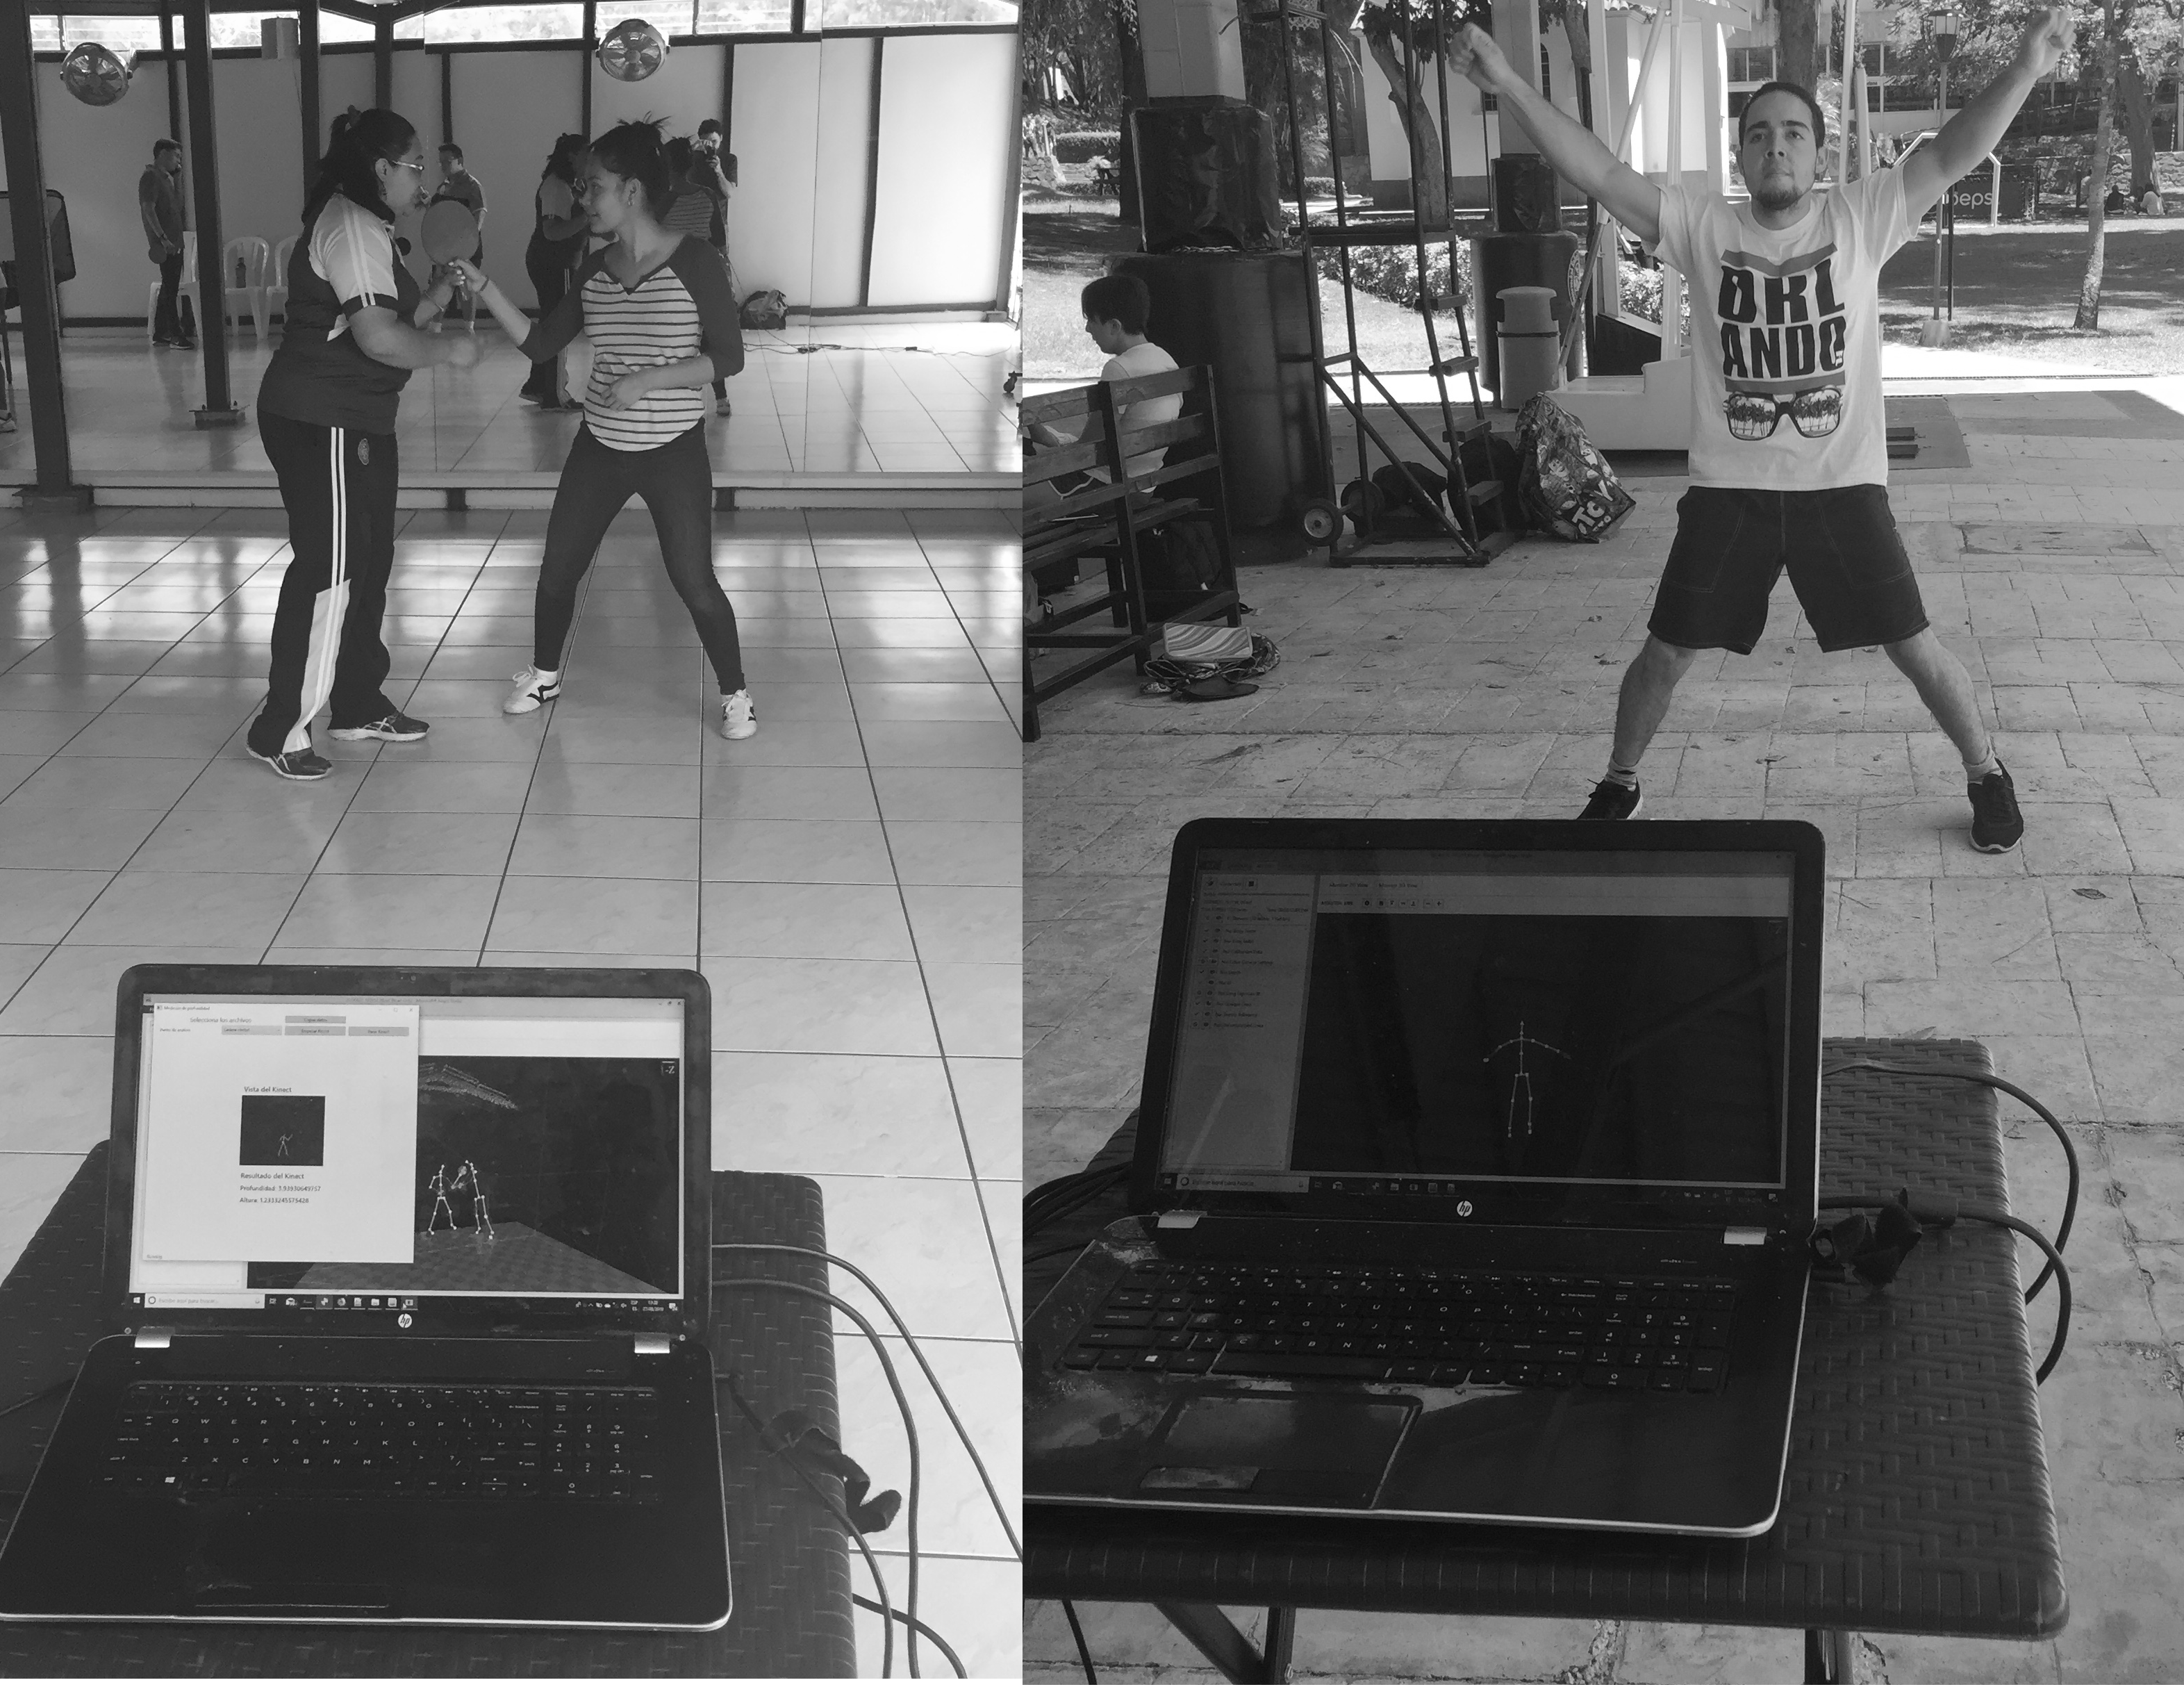
\includegraphics[width=280px,height=280px]{graphics/tomaDatos.png} \\
	\textbf{Fuente:} Propia
\end{figure} 
\subsection{Documentaci\'on del movimiento}
El investigador realiz\'o una breve entrevista a cada entrenador y algunos atletas (similar a un grupo focal), con la finalidad de detallar todos los aspectos de los movimientos, adem\'as de definir los pasos requeridos de cada movimiento v\'alido. Posteriormente a la entrevista, el investigador complet\'o todos los formularios respectivos de movimiento (Formularios de datos de entradas):
\subsubsection{Formularios de entradas de tenis de mesa}
\begin{figure}[H]
	\caption{Formulario de movimiento de tenis de mesa}
	\label{fig:frmMovTen}
	\centering	\includegraphics[width=445px,height=600px]{graphics/resultados/movimientoTenis.PNG} \\
	\textbf{Fuente:} Elaborado por el autor de tesis con base a las observaciones del trabajo de campo
\end{figure}
\begin{figure}[H]
	\caption{Formulario de rutina de tenis de mesa}
	\label{fig:frmRoutTen}
	\centering	\includegraphics[width=445px,height=600px]{graphics/resultados/rutina-tennis.PNG} \\
	\textbf{Fuente:} Propia
\end{figure}
\subsubsection{Formularios de entradas de animaci\'on}
\begin{figure}[H]
	\caption{Formulario de movimiento de animaci\'on}
	\label{fig:frmMovCheer}
	\centering	\includegraphics[width=445px,height=600px]{graphics/resultados/movimientoCheerleader.PNG} \\
	\textbf{Fuente:} Propia
\end{figure}
\begin{figure}[H]
	\caption{Formulario de rutina de animaci\'on}
	\label{fig:frmRoutCher}
	\centering	\includegraphics[width=400px,height=490px]{graphics/resultados/rutina-cheerleaders.PNG} \\
	\textbf{Fuente:} Propia
\end{figure}
\subsubsection{Formularios de entradas de taekwondo}
\begin{figure}[H]
	\caption{Formulario de movimiento taekwondo}
	\label{fig:frmWhiteMov}
	\centering	\includegraphics[width=445px,height=600px]{graphics/resultados/movimientoTaekwondo.PNG} \\
	\textbf{Fuente:} Propia
\end{figure}
\begin{figure}[H]
	\caption{Formulario de rutina de taekwondo}
	\label{fig:frmRoutTaek}
	\centering	\includegraphics[width=445px,height=600px]{graphics/resultados/rutina-taekwondo.PNG} \\
	\textbf{Fuente:} Propia
\end{figure}
\subsection{Etiquetaci\'on de v\'ideos}
El investigador cre\'o desde cero, una base de datos de gesturas por movimiento (a partir del instrumento Visual Gesture Builder), luego se adjunt\'o a la base de datos, todos los v\'ideos recuperados de la actividad de la toma de datos, y por cada v\'ideo se analiz\'o fotograma por fotograma, asignando un valor a cada paso del movimiento, tal como se muestra en la figura de proceso de etiquetaci\'on del movimiento:
 \begin{figure}[H]
	\caption{Proceso de etiquetaci\'on del movimiento derecha}
	\label{fig:getTag}
	\centering
	\includegraphics[width=250px,height=250px]{graphics/etiquetas.png} \\
	\textbf{Fuente:} Propia
\end{figure} 
\subsection{Construcci\'on y pruebas del modelo}
Por cada modelo, el investigador separ\'o los v\'ideos etiquetados en dos partes:
\begin{itemize}
\item \textbf{V\'ideos para el entrenamiento y construcci\'on del modelo:} Elementos que permiten  entrenar el modelo, generando un archivo de base de datos de gesturas (.gdb), la cual proporciona el valor del factor de movimiento a partir del algoritmo Random Forest Regression.
\item \textbf{V\'ideos para an\'alisis:} El investigador seleccion\'o el archivo de bases de datos de gesturas, y posteriormente la herramienta analiz\'o cada v\'ideo, proporcionando el valor real y pronosticado del modelo, tal como se muestra en la figura de obtenci\'on de valores, el valor real es de 0.008018661, mientras que el valor pronosticado es de \num{103893e-6}:
\end{itemize}
 \begin{figure}[H]
	\caption{Obtenci\'on del valor real y pronosticado}
	\label{fig:getError}
	\centering
	\includegraphics[width=300px,height=300px]{graphics/getError.png} \\
	\textbf{Fuente:} Propia
\end{figure} 
\subsection{Selecci\'on y aceptaci\'on del modelo}
\begin{itemize}
\item \textbf{Selecci\'on:} El investigador realiz\'o tres submodelos distintos por movimiento, con distintos datos de entrenamiento (combinaciones de v\'ideos de entrenamientos y an\'alisis). As\'i mismo por cada submodelo se analiz\'o un v\'ideo de an\'alisis, tabulando los datos reales y pronosticado en una hoja de observaciones (Ver anexos, tabla \ref{tab:obsErrores}). Posteriormente al proceso de tabulaci\'on, se calcul\'o los errores correspondientes de cada modelo (error medio pronosticado, desviaci\'on media absoluta y la ra\'iz del error cuadr\'atico medio), seleccionando as\'i el modelo que tenga un menor error. 
\item \textbf{Aceptaci\'on:} El investigador  verifica la media de los errores de cada submodelo, en caso que el error sea mayor o igual  a un medio del valor de reconocimiento (valor recuperado por los formularios del paso de documentaci\'on del movimiento) se rechaza el modelo, en caso contrario, se da la aprobaci\'on y se construye los intervalos de confianza de detecci\'on de los pasos de un movimiento v\'alido, adem\'as de calcular los porcentajes de detecci\'on de movimiento v\'alido e inv\'alido.
\end{itemize}
\subsection{Extracci\'on de datos de los v\'ideos}
Por cada modelo aceptado, el investigador extrajo los datos del tiempo y el recorrido de la mu\~neca derecha de una repetici\'on, con el fin de objetivo de validar que cada modelo fue entrenado con distintos datos, reflejado en una  regresi\'on de tiempo y recorrido. Lo cual para construir dicha regresi\'on, el investigador separ\'o por cada v\'ideo, los renglones de fotogramas de una repetici\'on, listando los tiempos iniciales y finales utilizado para la extracci\'on de datos de v\'ideos .xef (recuperado del instrumento, Kinect studio).
\begin{figure}[H]
	\caption{Segmentos de repeticiones de un v\'ideo}
	\label{fig:segVideo}
	\centering
	\includegraphics[width=420px,height=100px]{graphics/separarPuntos.PNG} \\
	\textbf{Fuente:} Propia
\end{figure} 
\subsection{Validaci\'on  del modelo en tiempo real}
El investigador realiz\'o una \'ultima visita a cada equipo deportivo (cuyo modelo fue aprobado), en dicha visita instal\'o el prototipo del modelo en lugar asignado (en paralelo, los atletas realizaban el calentamiento), posteriormente a la instalaci\'on, el investigador le ense\~n\'o al entrenador una versi\'on de prueba de una rutina tabata, dicha prueba lo realiz\'o el investigador (cabe resaltar que el investigador vest\'ia deportivamente y adem\'as ejecut\'o previamente los ejercicios de calentamiento) con una rutina de 1 serie de 10 segundos de descanso y 50 segundos de trabajo. Luego de la prueba, el entrenador seleccion\'o a un grupo de atletas que no participaron en el proceso de toma de datos, y posteriormente se le program\'o a cada atleta del grupo, una rutina tabata (cada deportista se posicion\'o en la distancia de profundidad recomendada).
 \begin{figure}[H]
	\caption{Fotograf\'ias durante la validaci\'on del modelo}
	\label{fig:getvalidationStep}
	\centering
	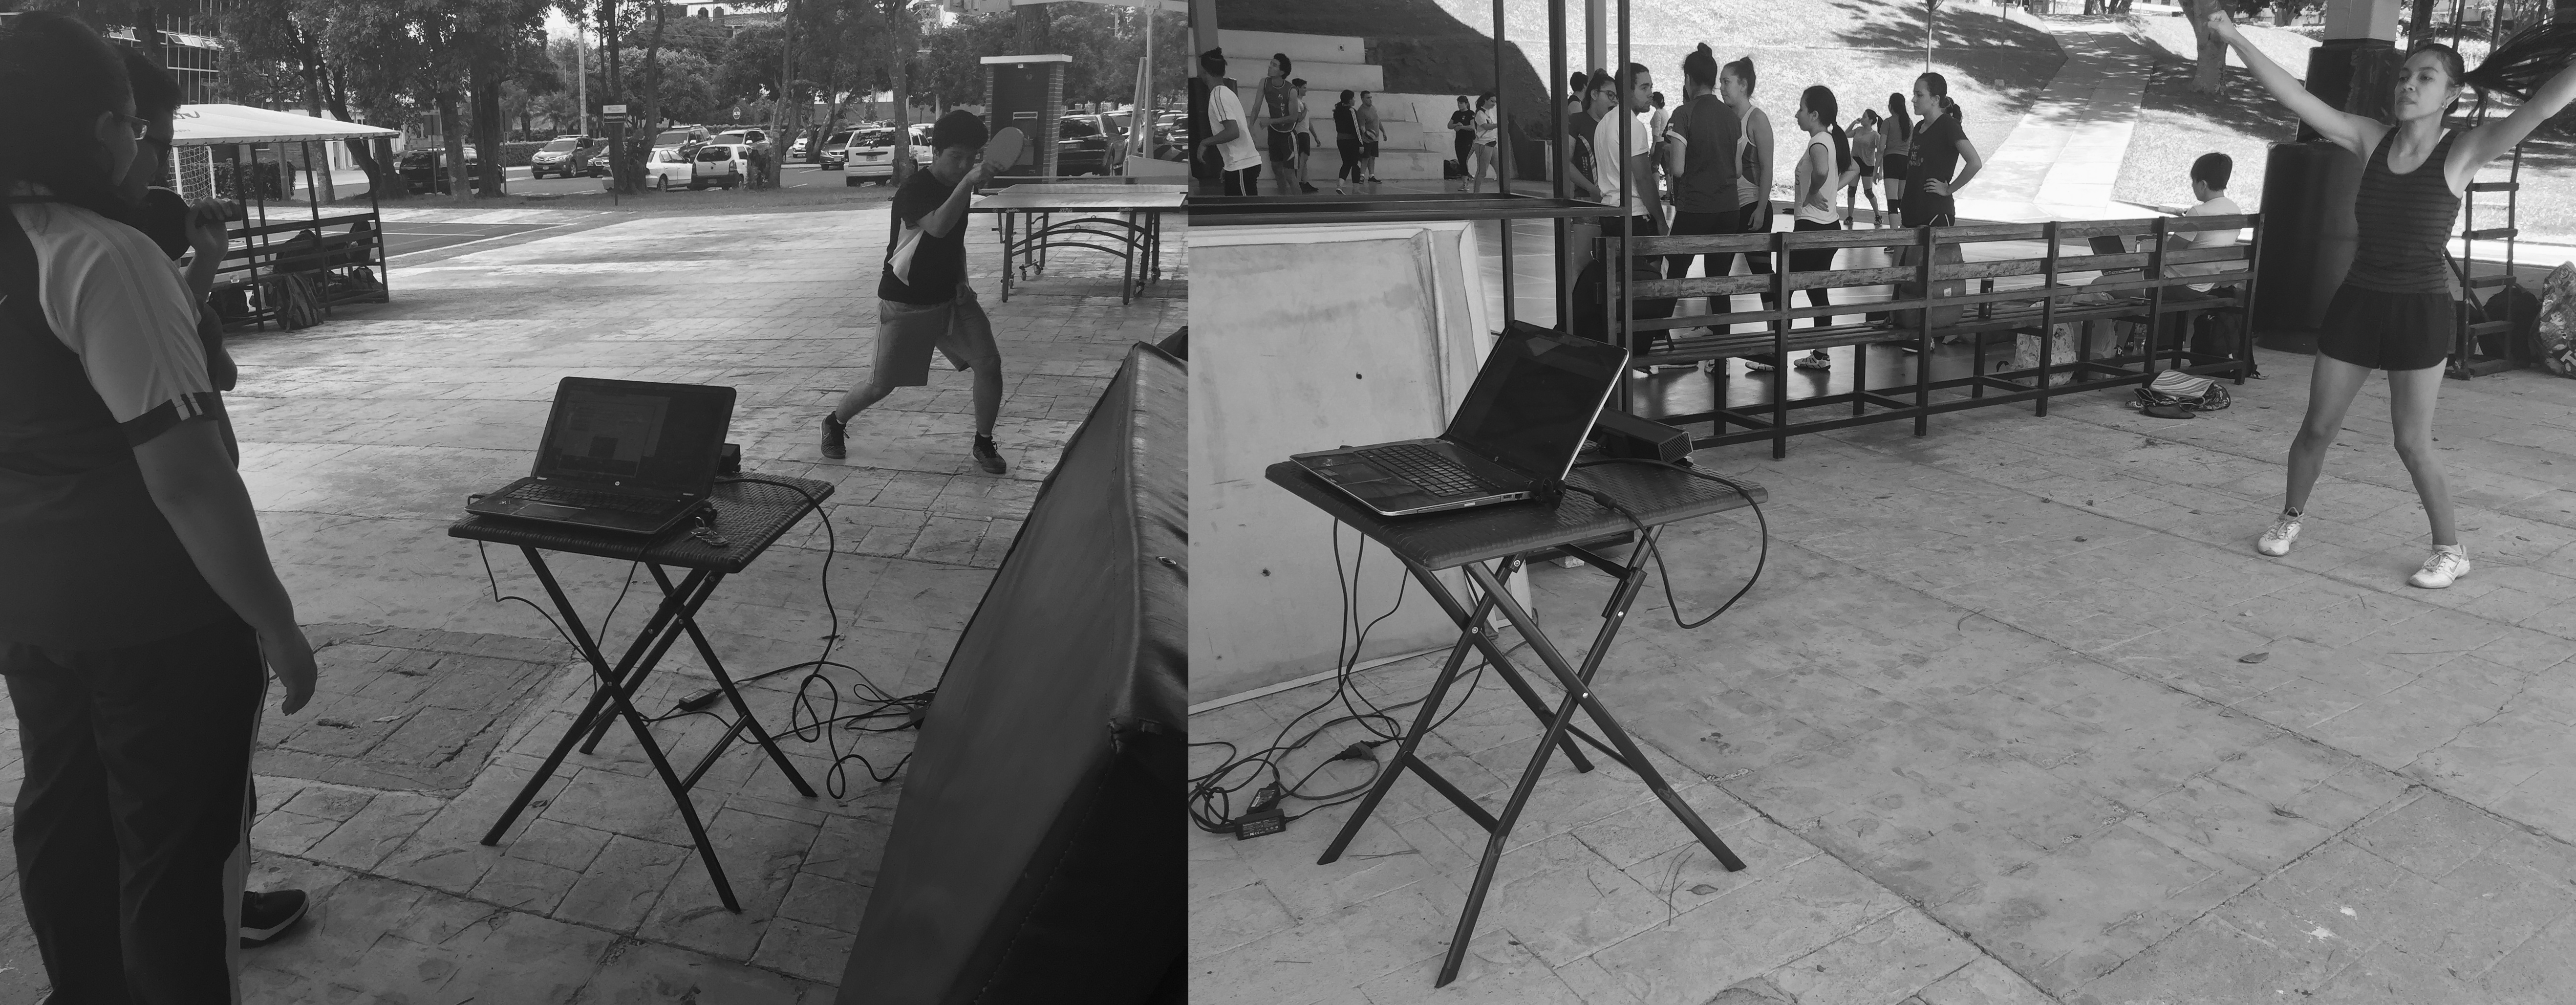
\includegraphics[width=165px,height=165px]{graphics/tabataResultados.png} \\
	\textbf{Fuente:} Propia
\end{figure} 
\section{Dise\~no de la metodolog\'ia}\label{dis}
Esta secci\'on se presenta todos los dise\~nos y c\'alculos matem\'aticos y estad\'isticos encontrados en los resultados. 
\subsection{Asignaci\'on de valores de etiquetas y rangos de identificaci\'on}\label{dis:asig}
Estos valores permiten identificar el paso de cada movimiento a partir de las siguientes variables:
\begin{itemize}
\item \textbf{Offset:} Valor de distribuci\'on de etiquetas de cada paso del movimiento, por partes iguales.
\begin{formula}[H]
	\centering
	\caption{Offset de etiquetas}
	\label{frm:offsetEt}
	\begin{equation}
offset = \frac{1}{pasos-1}
	\end{equation}
	\textbf{Fuente:} Propuesto por el autor de tesis
\end{formula}
\item \textbf{Vector de etiquetas:} A cada paso se le distribuye un valor \'unico, cuyo valor se calcula a partir del offset de la etiqueta anterior.
\begin{formula}[H]
	\centering
	\caption{Asignaci\'on de etiquetas}
	\label{frm:vecEtiq}
	\begin{equation}
\begin{matrix}
etiquetas=[0, etiqueta(1), ..., etiqueta(paso), ..., 1],\; donde
\\
\\
etiqueta(paso) =
\left\{\begin{matrix}
0 & Si\; es\; el\; primer \; paso
\\
etiqueta(paso-1)+offset & Si\; es\; un\; paso\; intermedio
\\ 
1 & Si\; es\; el\; \acute{u}ltimo\; paso
\end{matrix}\right.
\end{matrix}
	\end{equation}
	\textbf{Fuente:} Propuesto por el autor de tesis
\end{formula} 

\item \textbf{Valor de identificaci\'on:} N\'umero que representa la distribuci\'on de reconocimiento  de pasos por partes iguales:
\begin{formula}[H]
	\centering
	\caption{Valor de identificaci\'on de pasos}
	\label{frm:idenStep}
	\begin{equation}
valor \: de \: identificaci\acute{o}n = \frac{1}{pasos}
	\end{equation}
	\textbf{Fuente:} Propuesto por el autor de tesis
\end{formula} 

\item \textbf{Rango de identificaci\'on:} Rango m\'aximo num\'erico para identificar un paso.
\begin{formula}[H]
	\centering
	\caption{Rango m\'aximo de identificaci\'on de un paso}
	\label{frm:idenStep}
	\begin{equation}
\begin{matrix}
rango = [[inferior,superior]] \\
\\
rango(paso)=\left\{\begin{matrix}
inferior(paso)= \left\{\begin{matrix}
0 & paso\: inicial\\ 
superior(paso-1) & paso\: no\: inicial
\end{matrix}\right.\\ 
\\
superior(paso)= \left\{\begin{matrix}
inferior(paso)+identificaci\acute{o}n & paso\, no\, final\\ 
1 & paso\: final

\end{matrix}\right.\\ 
\end{matrix}\right.
\end{matrix}
	\end{equation}
	\textbf{Fuente:} Propuesto por el autor de tesis
\end{formula} 
\end{itemize}
\subsection{C\'alculo indirecto de la altura del usuario} \label{dis:height}
Para el presente proyecto se midi\'o la altura del usuario, a partir de la diferencia entre la altura de la cabeza y la altura promedio de los pies.
	\begin{formula}[H]
	\centering
	\caption{Altura del usuario}
	\label{frm:alturaUser}
	\begin{equation}
y_{usuario}=y_{cabeza}-\frac{y_{pie \: derecho}+y_{pie \: izquierdo}}{2}
	\end{equation}
			\textbf{Fuente:} Planteado por el autor de tesis
\end{formula} 
\subsection{C\'alculo de distancia de profundidad m\'inima y m\'axima} \label{dis:deep}
Para los siguientes c\'alculos se utilizaron la hoja de observaciones de profundidad (Ver anexo, tabla  \ref{tab:obsDepth}), aplicando las siguientes funciones de microsoft excel (versi\'on ingl\'es):
\begin{itemize}
       \item \textbf{Average}: Funci\'on para determinar la altura promedio.
\begin{formula}[H]
	\centering
	\caption{C\'alculo de altura promedio}
	\label{frm:avgHeight}
	\begin{equation}
	Altura \: promedio =AVERAGE([Altura])
	\end{equation}
		\textbf{Fuente:} Elaborado por el autor, a partir de funci\'on de excel
\end{formula}
       \item \textbf{Stdev}: Funci\'on para determinar la desviaci\'on est\'andar de la altura.
\begin{formula}[H]
	\centering
	\caption{C\'alculo de desviaci\'on est\'andar de la altura}
	\label{frm:stdevHeight}
	\begin{equation}
	desviaci\acute{o}n \:  de \: altura =STDEV([Altura])
	\end{equation}
		\textbf{Fuente:} Elaborado por el autor, a partir de funci\'on de excel
\end{formula}
       \item \textbf{Max}: Funci\'on para determinar la profundidad m\'axima entre el Kinect y el atleta.
       \begin{formula}[H]
	\centering
	\caption{C\'alculo de la profundidad m\'axima}
	\label{frm:maxDepth}
	\begin{equation}
	Profundidad \: Max =MAX([Profundidad])
	\end{equation}
		\textbf{Fuente:} Elaborado por el autor, a partir de funci\'on de excel
\end{formula}
       \item \textbf{Min}: Funci\'on para determinar la profundidad m\'inima entre el Kinect y el atleta.
              \begin{formula}[H]
	\centering
	\caption{C\'alculo de la profundidad m\'inima}
	\label{frm:minDepth}
	\begin{equation}
	Profundidad \:  Min =MIN([Profundidad])
	\end{equation}
		\textbf{Fuente:} Elaborado por el autor, a partir de funci\'on de excel.
\end{formula}
\end{itemize}
\subsection{Eventos del Kinect} \label{dis:even}
De acuerdo a la hoja de observaciones de extracci\'on de datos de v\'ideos (Ver tabla \ref{tab:obsVideoData}), se recupera la siguiente informaci\'on:
\begin{itemize}
\item \textbf{Eventos}: Conjunto de datos del seguimiento del esqueleto, durante un intervalo de tiempo.
\begin{formula}[H]
	\centering
	\caption{Matriz de eventos del Kinect}
	\label{frm:event}
	\begin{equation}
\begin{matrix}
Esqueleto & [SkeletonId, Joint, status, x, y, z] \\ 
Evento & [EventoIndex, TotalTime, esqueleto]  \\
\\ 
Eventos & 
\left.\begin{matrix}
Tiempo \: inicial\\ 
\\ 
\\
Tiempo \: final
\end{matrix}\right\}
\begin{matrix}
\left.\begin{matrix}
Evento \: inicial 
\end{matrix}\right\}\\ 
\left.\begin{matrix}
.. \\ 
Eventos \: no \: iniciales \\ 
 ..
\end{matrix}\right\}
\end{matrix}
\begin{bmatrix}
Evento_{0}\\ 
Evento_{1}\\ 
Evento_{2}\\ 
Evento_{x}
\end{bmatrix}
\end{matrix}
	\end{equation}
		\textbf{Fuente:} Propuesto por el autor de tesis.
\end{formula}
\item \textbf{Tiempo relativo}: Describe el tiempo de la repetici\'on, cuyo valor significa la diferencia entre el tiempo total de un evento no inicial y el tiempo total del primer evento.
              \begin{formula}[H]
	\centering
	\caption{C\'alculo del tiempo de la repetici\'on}
	\label{frm:relativeTime}
	\begin{equation}
	relative \: time = TotalTime_{Evento\: x}-TotalTime_{Evento\: inicial}
	\end{equation}
		\textbf{Fuente:} Propuesto por el autor de tesis.
\end{formula}
\item \textbf{Distancia euclidiana}: Describe el desplazamiento de una articulaci\'on, bas\'andose en la posici\'on del primer evento inicial y la posici\'on de un evento no inicial:
\begin{formula}[H]
	\centering
	\caption{Desplazamiento de una articulaci\'on}
	\label{frm:desplazaUser}
	\begin{equation}
|r|=\sqrt{(x_{joint}-x_{o})^{2}+(y_{joint}-y_{o})^{2}+(z_{joint}-z_{o})^{2}}
	\end{equation}
	\textbf{Fuente:} Distancia euclidiana \cite[p.~423]{ayres2001calculo}
\end{formula}  
\end{itemize}
\subsection{Captura de datos durante una rutina (normalizaci\'on de datos)}\label{dis:recognitionMove}
Durante la rutina, los datos del seguimiento del esqueleto son recuperados a partir del kit de desarrollo de software del Kinect, dichos datos son almacenados en la siguiente estructura:
\begin{itemize}
\item \textbf{I:} Valor num\'erico \'unico que identifica una articulaci\'on.
\item \textbf{X:} Posici\'on horizontal de la articulaci\'on, dibujado en una imagen de dos dimensiones.
\item \textbf{Y:} Posici\'on vertical de la articulaci\'on, dibujado en una imagen de dos dimensiones.
\item \textbf{Fm:} Factor del movimiento proporcionado por la base de datos de gesturas.
\item \textbf{P:} Valor num\'erico que identifica el paso que est\'a realizando un atleta.
\item \textbf{Tiempo:} Tiempo de captura de datos.
\item \textbf{Joint:} Vector que almacena la posici\'on de una articulaci\'on en una figura de dos dimensiones.
\item \textbf{Esqueleto:} Vector que almacena todos los vectores de articulaciones del esqueleto humano.
\item \textbf{Step:} Vector que almacena informaci\'on del seguimiento del esqueleto, factor del movimiento y el tiempo de un paso.
\item \textbf{Repetici\'on:} Vector que almacena la informaci\'on de cada de paso de un movimiento.
\item \textbf{Serie:} Vector que almacena las repeticiones del movimiento durante una serie.
\item \textbf{Series:} Vector que almacena la informaci\'on de cada serie de la rutina.
\end{itemize}
\begin{formula}[H]
	\centering
	\caption{Matriz de datos capturados durante una rutina}
	\label{frm:MatrizDatosRepeticion}
	\begin{equation}
\begin{matrix}
i & enumerador\: de\: la\: articulaci\acute{o}n \\ 
x & distancia\, horizontal \: (p\acute{i}xeles) \\ 
y & distancia\, vertical\: (p\acute{i}xeles) \\ 
joint_{i}& [i,x,y] \\ 
 & \\ 
esqueleto & \begin{bmatrix}
joint_{0} \\ 
... \\ 
joint_{i}\\ 
... \\ 
joint_{24}
\end{bmatrix}  \\ 
 & \\ 
fm & factor \, del \, movimiento \\ 
p  & paso \, del \,movimiento \\ 
t  & tiempo \, total \\ 
step_{p}  & [fm,p,esqueleto, tiempo] \\
 & \\ 
Repeticion & [step_{0}, ...,  step_{col}, ..., step_{last}] \\
serie & [repeticion] \\
series & [serie]
\end{matrix}
	\end{equation}
	\textbf{Fuente:} Propuesto por el autor de tesis
\end{formula}
\subsection{Validaci\'on del modelo de reconocimiento de movimiento}\label{dis:validate}
El presente proyecto se utiliz\'o dos m\'etodos de validaciones cruzadas \cite{perez2015analisis}:
\begin{itemize}
\item \textbf{Hold out:} Las muestras de datos se separan en dos conjunto, uno para construir y entrenar el modelo -i.e. Build- y otro para realizar pruebas que dan validez a los m\'argenes  de errores del modelo.
\item \textbf{K-fold:} Las muestras se dividen en K subconjuntos, y en cada subconjunto se aplica el m\'etodo hold out.
\end{itemize}  
\begin{table}[H]
\begin{center}
\caption{Validaci\'on cruzada, 3-fold de tenis de mesa}
\label{tab:KfoldTenis}
\begin{tabular}{|l|l|l|}
\hline
\multicolumn{3}{|c|}{\textbf{Muestra de v\'ideos}} \\ \hline
\multicolumn{3}{|c|}{1, 2, 3, 4, 5, 6} \\ \hline
\textbf{Modelo} & \textbf{Builds} & \textbf{Test} \\ \hline
1 & 1, 2, 3, 4, 5 & 6 \\ \hline
2 & 1, 2, 4, 5, 6 & 3 \\ \hline
3 & 2, 3, 4, 5, 6 & 1 \\ \hline
\multicolumn{3}{l}{\textbf{Fuente:} Propia}
\end{tabular}
\end{center}
\end{table}
\begin{table}[H]
\begin{center}
\caption{Validaci\'on cruzada, 3-fold de animaci\'on}
\label{tab:KfoldAnimacion}
\begin{tabular}{|l|l|l|}
\hline
\multicolumn{3}{|c|}{\textbf{Muestra de v\'ideos}} \\ \hline
\multicolumn{3}{|c|}{1, 2, 3, 4, 5, 6, 7} \\ \hline
\textbf{Modelo} & \textbf{Builds} & \textbf{Test} \\ \hline
1 & 1, 2, 3, 4, 5, 6 & 1 \\ \hline
2 & 1, 2, 3, 5, 6, 7 & 4 \\ \hline
3 & 1, 2, 3, 4, 5, 6 & 7 \\ \hline
\multicolumn{3}{l}{\textbf{Fuente:} Propia}
\end{tabular}
\end{center}
\end{table}
\begin{table}[H]
\begin{center}
\caption{Validaci\'on cruzada, 3-fold de taekwondo}
\label{tab:KfoldTaekwondo}
\begin{tabular}{|l|l|l|}
\hline
\multicolumn{3}{|c|}{\textbf{Muestra de videos}} \\ \hline
\multicolumn{3}{|c|}{1, 2, 3, 4, 5, 6, 7, 8, 9, 10, 11, 12, 13, 14, 15, 16} \\ \hline
\textbf{Modelo} & \textbf{Builds} & \textbf{Test} \\ \hline
1 & 1, 2, 3, 4, 5, 6, 7, 8, 9, 11, 12, 13, 14, 15, 16 & 10 \\ \hline
2 & 1, 2, 3, 4, 5, 6, 7, 8, 9, 10, 12, 13, 14, 15, 16 & 11 \\ \hline
3 & 1, 2, 3, 4, 5, 6, 7, 8, 9, 10, 11, 13, 14, 15, 16 & 12 \\ \hline
\multicolumn{3}{l}{\textbf{Fuente:} Propia}
\end{tabular}
\end{center}
\end{table}
Posteriormente en la etapa de pruebas, se realiz\'o  por cada modelo una hoja de observaciones de valores reales y pronosticados (ver anexo, tabla \ref{tab:obsErrores}), de modo de encontrar los siguientes errores de pron\'osticos \cite{erroresPronostico}:
\begin{itemize}
\item \textbf{Error medio pronosticado (\acrshort{EMP}):} Promedio de diferencia entre el valor real y pronosticado, la cual puede tener tres interpretaciones distintas:
	\begin{itemize}
	\item \textbf{Valor positivo:} En promedio, los valores pronosticado est\'an por debajo de los valores reales.
	\item \textbf{Valor negativo:} En promedio, los valores pronosticado est\'an por arriba de los valores reales.
	\item \textbf{Valor cero:} Los valores pronosticados pueden estar por debajo o por arriba de los valores reales.
	\end{itemize}
\begin{formula}[H]
	\centering
	\caption{C\'alculo del error medio pronosticado}
	\label{frm:empMath}
	\begin{equation}
EMP=\frac{\sum_{0}^{n}(Real_{x}-Pronostic_{x}\cdot10^{-6})}{n}
	\end{equation}
	\textbf{Fuente:} Formula adaptada al proyecto, a partir de la f\'ormula del error medio pronosticado \cite{videoErrores}
\end{formula}  
\item \textbf{Desviaci\'on media absoluta (\acrshort{DMA}):} Promedio de diferencia absoluta entre el valor real y pronosticado, que muestra la dispersi\'on con respecto al valor real.
 \begin{formula}[H]
	\centering
	\caption{C\'alculo de la desviaci\'on media absoluta}
	\label{frm:MADMath}
	\begin{equation}
DMA=\frac{\sum_{0}^{n}( \left |  Real_{x}-Pronostic_{x}\cdot10^{-6} \right |)}{n}
	\end{equation}
	\textbf{Fuente:} Formula adaptada al proyecto, a partir de la f\'ormula de la desviaci\'on media absoluta \cite{videoErrores}
\end{formula}  
\item \textbf{Ra\'iz del error cuadr\'atico medio (RECM):} Es la desviaci\'on est\'andar de los errores de predicci\'on, la cual indica qu\'e tan disperso se encuentra los errores con respecto al error medio pronosticado.
 \begin{formula}[H]
	\centering
	\caption{C\'alculo de la ra\'iz del error cuadr\'atico medio}
	\label{frm:RECMMath}
	\begin{equation}
RECM=\sqrt{\frac{\sum_{0}^{n}((Real-Pronostic\cdot10^{-6})-EMP)^{2}}{n}}
	\end{equation}
	\textbf{Fuente:} Formula adaptada al proyecto, a partir de la f\'ormula de la ra\'iz del error cuadr\'atico medio \cite{GEORCMETUT}
\end{formula}  
\end{itemize}
Luego de encontrar los errores, se debe seleccionar el modelo que tenga la menor \acrshort{RECM}, y posteriormente encontrar los errores de la muestra total:
 \begin{formula}[H]
	\centering
	\caption{EMP de la muestra total}
	\label{frm:EmpAll}
	\begin{equation}
EMP_{muestra\, total}=AVERAGE([EMP_{modelo}])
	\end{equation}
	\textbf{Fuente:} Propuesto por el autor de tesis, con base a las f\'ormulas de excel (versi\'on en ingl\'es)
\end{formula}  
 \begin{formula}[H]
	\centering
	\caption{MAD de la muestra total}
	\label{frm:MadAll}
	\begin{equation}
MAD_{muestra\, total}=AVERAGE([MAD_{modelo}])
	\end{equation}
	\textbf{Fuente:} Propuesto por el autor de tesis, con base a las f\'ormulas de excel (versi\'on en ingl\'es)
\end{formula}  
	 \begin{formula}[H]
	\centering
	\caption{RECM de la muestra total}
	\label{frm:RecmAll}
	\begin{equation}
RECM_{muestra\, total}=AVERAGE([RECM_{modelo}])
	\end{equation}
	\textbf{Fuente:} Propuesto por el autor de tesis, con base a las f\'ormulas de excel (versi\'on en ingl\'es)
\end{formula} 
Los errores de la muestra total ayudan aceptar o rechazar el modelo; si la \acrshort{RECM} promedio  es menor a un medio del valor de identificaci\'on se aprueba (se divide entre dos, debido que las etiquetas de los pasos intermedio se encuentra a la mitad de cada rango de identificaci\'on respectiva). En caso que sea mayor o igual, se rechaza, debido que los intervalos de confianza colisiona con otros intervalos de confianza (Intervalos que se utiliza para la detecci\'on de un paso):
\begin{figure}[H]
	\caption{Criterios de aceptaci\'on de un modelo de detecci\'on de los pasos requeridos de un movimiento}
	\label{fig:AproveOrDennie}
	\centering
	\includegraphics[width=430px,height=360px]{graphics/CriterioAceptacion.png} \\
	\textbf{Fuente:} Propia
\end{figure}
En la figura \ref{fig:AproveOrDennie}, se separa en tres partes:
\begin{itemize}
\item \textbf{Detalles generales del movimiento:} Muestra las variables num\'ericas de un movimiento.
\item \textbf{Caso aprobado:} Al construir los intervalos de confianza, se observa que no colisiona entre s\'i.
\item \textbf{Caso rechazado:} Al construir los intervalos de confianza, se observa que los intervalos del paso 1 colisiona con el paso 2 (debido que el intervalo de confianza inferior del paso 2 se encuentra dentro del intervalo de confianza del paso 1), y los intervalos del paso 2 colisiona con el paso 3 (debido que el intervalo de confianza inferior del paso 3 se encuentra dentro del intervalo de confianza del paso 2).
\end{itemize}
Adem\'as, por cada modelo aprobado se debe encontrar los intervalos de confianza  que permite detectar los pasos de un movimiento v\'alido:
\begin{formula}[H]
	\centering
	\caption{Intervalos de confianza de reconocimiento de un paso}
	\label{frm:rangoConfiabilidad}
	\begin{equation}
\begin{matrix}

intervalo\: de\: confianza = ic =[[inferior,superior]] \\
\\
ic(paso)=\left\{\begin{matrix}
inferior(paso)=\left\{\begin{matrix}
0 & si\, es\, el\, primer\, paso\\ \\ 
etiqueta(paso)- RECM_{muestra\, total} & si\: es\: paso\: intermedio \\ 
\\
1-RECM_{muestra\, total}& si\, es\, el\, \acute{u}ltimo\, paso
\end{matrix}\right. \\ 
\\ 
inferior(paso)=\left\{\begin{matrix}
RECM_{muestra\, total}& si\, es\, el\, primer\, paso \\
\\
etiqueta(paso)+RECM_{muestra\, total} & si\: es\: paso\: intermedio \\ \\ 
1 & si\: es\: el\: \acute{u}ltimo\: paso
\end{matrix}\right.
\end{matrix}\right.
\end{matrix}
	\end{equation}
	\textbf{Fuente:} Propuesto por el autor de tesis
\end{formula} 
Por otro lado, se debe determinar el valor de recognition, n\'umero porcentual que determina el porcentaje de detecci\'on similar al fotograma de cada paso respectivo, es decir:
 \begin{itemize}
\item \textbf{Porcentaje mayor a cero:} Entre m\'as cercano al 100\%, el factor de movimiento es similar al valor de etiquetado (menor error).
\item \textbf{Porcentaje menor o igual a cero:} Son modelos rechazado, debido que el error es grande y adem\'as no detecta los pasos de un movimiento (por colisiones de los intervalos de confianza).
\end{itemize}
\begin{formula}[H]
	\centering
	\caption{Valor de recognition}
	\label{frm:Recognitiona}
	\begin{equation}
recognition=1-no\,v\acute{a}lidos=1-\frac{RECM_{muestra\, total}}{valor\: de\: identificaci\acute{o}n}  
	\end{equation}
	\textbf{Fuente:} Propuesto por el autor de tesis
\end{formula}
\subsection{Algoritmo clasificador de un movimiento v\'alido}\label{dis:algoritmoDet}
Se presenta el algoritmo clasificador de repetici\'on de un movimiento v\'alido:
\begin{itemize}
\item Entradas:
\begin{itemize}
\item \textbf{Paso siguiente:} Variable que lleva el control del orden de todos los pasos detectados.
\item \textbf{Factor del movimiento:} Variable que indica la transici\'on del movimiento a partir del algoritmo Random Forest Regression.
\item \textbf{Paso detectado:} Variable que indica el paso actual del factor del movimiento.
\item \textbf{Paso no detectado:} Variable que no tiene un valor al inicio, la cual se asigna un valor en el caso que sea una repetici\'on inv\'alida (indica el paso del fallo del movimiento).
\end{itemize}
\item Procesos:
\begin{enumerate}[1.]
\item Asignar el paso siguiente como paso inicial (paso No.1), debido que marca el inicio de la repetici\'on. %1
\item Capturar un nuevo fotograma del Kinect, y obtiene el factor del movimiento del respectivo fotograma, a partir del algoritmo Random Forest Regression y la herramienta, Visual Gesture Builder. %2
\item Verificar si el factor del movimiento se encuentra en alg\'un intervalo de confianza para obtener el paso detectado, en caso que no se encuentre, no devolver\'a ning\'un valor.  %3
\item Verificar si el paso detectado tiene un valor, adem\'as de chequear que no sea un valor anterior (valor anterior del paso siguiente), en caso que no cumpla ambas condiciones, se debe esperar a capturar un nuevo fotograma (Volver al proceso No.2). %4
\item Verificar si el paso detectado es igual al paso siguiente, en caso que sea diferente se detect\'o una repetici\'on inv\'alida (saltar al proceso No. 9). %5
\item Verificar si el paso detectado es el \'ultimo paso, en caso contrario (saltar al proceso No. 8) %6
\item Finalizar algoritmo con repetici\'on v\'alida. %7 
\item Incrementar el paso siguiente y volver a obtener un nuevo fotograma del Kinect (saltar al proceso No. 2). %8
\item Asignar el paso no detectado como paso siguiente.
\item Finalizar el algoritmo con repetici\'on inv\'alida.
\end{enumerate}
\item Salidas:
\begin{itemize}
\item \textbf{Repetici\'on v\'alida:} El usuario pas\'o por todos los pasos de un movimiento v\'alido de forma ordenada.
\item \textbf{Repetici\'on inv\'alida y su paso no detectado:} El usuario se salt\'o el paso no detectado, lo cual genera un movimiento inv\'alido.
\end{itemize}
\end{itemize}
\begin{figure}[H]
	\caption{Algoritmo clasificador de repetici\'on de un movimiento v\'alido }
	\label{fig:capturaDatos}
	\centering
	\includegraphics[width=430px,height=630px]{graphics/flujoGramaRepiticion.png} \\
	\textbf{Fuente:} Propia.
\end{figure}
Este algoritmo es aplicado para analizar los v\'ideos de testeos, debido que se etiquetaron  repeticiones de movimientos v\'alidos.  Sin embargo, al comparar los factores del movimiento de los fotogramas (de los v\'ideos de testeos), pueden ocurrir que no reconozca un paso, por lo tanto la repetici\'on del movimiento v\'alido se convierte en inv\'alido:
 \begin{figure}[H]
	\caption{Clasificaci\'on de repeticiones de movimiento v\'alido o inv\'alido  en un v\'ideo de testeo}
	\label{fig:detValido}
	\centering
	\includegraphics[width=430px,height=450px]{graphics/reconocimientoDePasos.png} \\
	\textbf{Fuente:} Propia.
\end{figure}
En la figura \ref{fig:detValido}, se divide en tres partes:
\begin{itemize}
\item \textbf{Intervalos de confianza:} Tabla que permite reconocer los pasos del movimiento, si el factor del movimiento se encuentra dentro del intervalo de confianza.
\item \textbf{Repetici\'on v\'alida:} Es v\'alido,  ya que detecta todos los pasos de manera ordenada  durante los fotogramas: Uno, tres y seis (observe que los factores del movimiento se encuentran dentro del alg\'un intervalo de confianza). 
\item \textbf{Repetici\'on inv\'alida:} Es inv\'alido, debido que para el fotograma 6, se esperaba detectar el paso dos (paso siguiente), pero se detect\'o el paso tres, por lo tanto el algoritmo determina que es una repetici\'on inv\'alida.
\end{itemize}
Este procedimiento permite completar la tabla de observaciones de clasificaci\'on de cada v\'ideo de testeo (ver anexos, tabla \ref{tab:DetectarPasoCorrecto}), en donde por cada repetici\'on etiquetada se verifica todos los pasos, por medio de tres valores:
\begin{itemize}
\item \textbf{Verdadero:} Si se detect\'o el paso correspondiente (de manera ordenada).
\item \textbf{Falso:} Repetici\'on invalida debido que no se detect\'o el paso correspondiente. 
\item \textbf{Sin valor:} El algoritmo no determin\'o ning\'un valor, debido que finaliz\'o al momento  que detect\'o una repetici\'on inv\'alida.
\end{itemize}
Por otra parte, se puede determinar el porcentaje de v\'alido e inv\'alidos del modelo de clasificador de repeticiones, adem\'as de determinar el porcentaje de cada paso no detectado:
\begin{formula}[H]
	\centering
	\caption{Porcentajes del modelo de clasificador}
	\label{frm:porcentajeClasificador}
	\begin{equation}
\begin{matrix}
repeticiones\: v\acute{a}lidas = contarSi(\acute{u}ltimo\: paso\: es\: verdadero) \\ 
 \\ 
repeticiones\: inv\acute{a}lidas = repeticiones\; totales\: del\: video - repeticiones\: v\acute{a}lidas\\ 
 \\ 
\%_{v\acute{a}lidos}=\frac{repeticiones\: v\acute{a}lidas}{repeticiones\; totales\: del\: video}\\ 
\\
\%_{inv\acute{a}lidos}=\frac{repeticiones\: inv\acute{a}lidas}{repeticiones\; totales\: del\: video}\\ 
\\ 
\%_{paso\; no\; detectado}=\frac{contarSi(paso\: es\: falso)}{repeticiones\: inv\acute{a}lidas}\\ 
\end{matrix}
	\end{equation}
	\textbf{Fuente:} Propuesto por el autor de tesis
\end{formula}
Es importante saber si el modelo de clasificaci\'on  de un movimiento v\'alido se aprueba, por lo tanto se debe calcular los porcentajes de referencias v\'alido e inv\'alido, que se determinan a partir del peor de los casos (detecta una repetici\'on v\'alida y las posibles combinaciones de una  repetici\'on inv\'alida): 
 \begin{figure}[H]
	\caption{Porcentajes de referencias v\'alidos e inv\'alidos }
	\label{fig:porcValido}
	\centering
	\includegraphics[width=430px,height=300px]{graphics/porceRef.png} \\
	\textbf{Fuente:} Propia.
\end{figure}
A partir de los porcentajes de referencias de clasificaci\'on, se pueden presentar dos casos:
\begin{itemize}
\item \textbf{Clasificaci\'on Aceptable:} Si el porcentaje de detecci\'on v\'alida es mayor al porcentaje de referencia v\'alida (Por consiguiente el porcentaje de detecci\'on inv\'alida es menor al porcentaje de referencia inv\'alida).
\item \textbf{Clasificaci\'on no aceptable:} Si el porcentaje de detecci\'on v\'alida es menor o igual al porcentaje de referencia v\'alida (Por consiguiente el porcentaje de detecci\'on inv\'alida es mayor o igual al porcentaje de referencia inv\'alida). 
\end{itemize}
\subsection{Dise\~no de los resultados de una rutina tabata} \label{dis:results}
En esta secci\'on se determina los resultados de la rutina de tabata, dichos resultados son encontrados a partir del seguimiento del esqueleto, la cual proporciona informaci\'on de las variables de los detalles del paso y repetici\'on (Ver f\'ormula \ref{frm:MatrizDatosRepeticion}), con el fin objetivo de encontrar la siguiente informaci\'on:
\begin{itemize}
\item \textbf{Volumen de repeticiones:} Sumatoria de las cantidades totales de repeticiones de una serie.  
\begin{code}[H]
	\caption{Pseudoc\'odigo para obtener las repeticiones totales de una rutina}
	\label{code:getRepetitions}
	\begin{lstlisting}
Entradas:
	Series de repeticiones del movimiento
	Contador de Repeticiones

Procesos:
	Recorrer cada serie de repeticiones del movimiento:
		Contar las repeticiones de la serie
		Sumar al contador de repeticiones

Salida:
	Contador de repeticiones
	\end{lstlisting}
	\textbf{Fuente:} Propia.
\end{code}

\item \textbf{Duraci\'on:} Tiempo total que se emplea en una rutina, tomando en cuenta todas las series de trabajos y descansos.
\begin{formula}[H]
	\centering
	\caption{C\'alculo de la duraci\'on de tiempo de una rutina}
	\label{eq:DurationTime}
	\begin{equation}
	Duration = \sum_{i=0}^{series}restTime +\sum_{i=0}^{series}workTime = series(restTime+workTime)
	\end{equation}
		\textbf{Fuente:} Elaborado por el autor de tesis
\end{formula}
\item \textbf{Resistencia:} Construye la estructura de la gr\'afica de la resistencia de un atleta durante una rutina a partir del recorrido de todas la series, posteriormente en cada serie se recorre todas las repeticiones y luego en cada repetici\'on se almacena el tiempo acumulado de la rutina y la cantidad de repeticiones que lleva el atleta a ese momento.
\begin{code}[H]
	\caption{Pseudoc\'odigo para crear la gr\'afica de resistencia}
	\label{code:getEndurance}
	\begin{lstlisting}
Entradas:
	Series de repeticiones del movimiento
	Gráfico en donde almacena
		Subgráfico que está compuesto por
			Nombre de la serie
			Listado de puntos en donde cada punto
				Guarda el tiempo (eje x)
				Guarda el numero de repetición (eje y)
	
Proceso:
	Crear gráfico
	Recorrer cada serie de repeticiones del movimiento
		Crear subgráfico
		Obtener el número de serie
		Crear el listado de puntos
		Recorrer cada repetición de la serie
			Obtener el número de repeticiones acumuladas 
			Obtener el tiempo del paso final de la repetición
			Crear un punto
			Guardar punto en el listado de puntos
		Almacenar en el subgráfico el número de serie y listado de puntos
		Guardar subgráfico en el listado que tiene el gráfico

Salida:
	Gráfico de resistencia
	\end{lstlisting}
	\textbf{Fuente:} Propia.
\end{code} 

\item \textbf{Potencia:} Resultado que muestra la cantidad m\'axima de repeticiones en el menor tiempo posible, la cual se encuentra a partir del recorrido de las series, luego en cada serie se determina la cantidad de repeticiones totales y el tiempo acumulado de la \'ultima repetici\'on, encontrando: 
	\begin{itemize}
	\item Una mayor cantidad de repeticiones almacenada anteriormente
	\item La misma cantidad de repeticiones almacenada anteriormente, pero se verifica si el tiempo acumulado es menor.
	\end{itemize}
\begin{code}[H]
	\caption{Pseudoc\'odigo para obtener la potencia}
	\label{code:getEndurance}
	\begin{lstlisting}
Entradas:
	Series de repeticiones del movimiento
	Potencia en donde almacena
		Cantidad de repeticiones acumuladas de una serie
		Tiempo total de la última repetición de la serie
		
Procesos:
	Crear potencia
	Recorrer cada serie de repeticiones del movimiento
		Obtener la última repetición de la serie
			Obtener el número de repeticiones acumuladas
			Obtener el tiempo del paso final de la repetición
			¿El número de repeticiones acumuladas aumentó?
				Si
					Almacenar los datos en potencia
				Sino si, ¿El número de repeticiones permaneció igual?:
					¿El Tiempo total disminuyó?:
						Si
							Almacenar los datos en potencia
						
Salida:
	Potencia 
	\end{lstlisting}
	\textbf{Fuente:} Propia.
\end{code} 

\item \textbf{Velocidad}: Raz\'on de cambio separado por:
	\begin{itemize}
	\item \textbf{Repeticiones por serie:} Variable que se determina a partir del promedio total de repeticiones por serie.
		\item \textbf{Tiempo por repetici\'on:} Variable que se determina a partir del promedio de la diferencia entre el tiempo del paso final y tiempo del paso inicial -i.e. Tiempo de una repetici\'on- de cada repetici\'on realizada por el atleta.
	\end{itemize}
\end{itemize}


\begin{code}[H]
	\caption{Pseudoc\'odigo para obtener las velocidades de las rutinas}
	\label{code:getTimeOfRepetitions}
	\begin{lstlisting}
Entradas:
	Series de repeticiones del movimiento
	Velocidad en donde almacena
		Repeticiones por serie
		Tiempo por serie
		
Proceso:
	Crear velocidad
	Crear un listado de tiempos de repeticiones
	Crear un listado de repeticiones de series
	Recorrer cada serie de repeticiones del movimiento
		Obtener el total de repeticiones de la serie
		Agregar al listado de repeticiones de series
		Recorrer cada repetición de la serie
			Obtener el tiempo del paso inicial de la repetición
			Obtener el tiempo del paso final de la repetición
			Encontrar la diferencia de tiempos del paso final e inicial
			Almacenar en el listado de tiempos de repeticiones
	Encontrar el promedio de repeticiones de series
	Transformar a número entero el promedio de repeticiones de series
	Encontrar el promedio de tiempos de repeticiones
	Almacenar ambos promedios en velocidad
	
Salida:
	Velocidad
	\end{lstlisting}
	\textbf{Fuente:} Propia.
\end{code} 
\section{Criterios del proyecto}\label{criter}
En esta secci\'on se presenta todos los criterios que se siguieron para crear el modelo de reconocimientos de movimientos:
\subsection{Criterios de selecci\'on de movimiento}
\begin{itemize}
	\item El investigador y el entrenador de cada deporte  seleccionaron aquellos movimientos que se ejecutan dentro del \'area de visi\'on del sensor Kinect.
	\item El movimiento no debe ser complejo, es decir que cualquier persona pueda realizar dicho movimiento, sin importar su nivel deportivo.
	\item Debe ser un movimiento que se emplea constantemente en el deporte, para aprender nuevos movimientos complejos.
\end{itemize}
\subsection{Criterios de an\'alisis de movimiento}
\begin{itemize}
	\item Cada movimiento debe tener una articulaci\'on de an\'alisis.
	\item El conjunto de articulaciones que interact\'uan en el movimiento, se debe seleccionar con base a la separaci\'on del cuerpo humano, es decir, la parte inferior (Articulaciones abajo de la cadera central) o superior (Articulaciones arriba de la cadera central).
\end{itemize}
\subsection{Criterios de etiquetaci\'on de movimiento}
\begin{itemize}
	\item Cada repetici\'on del movimiento debe pasar por todos los pasos.
	\item El rango de etiquetaci\'on debe estar entre valores de 0 (paso inicial) y 1 (paso final).
	\item La curva de aprendizaje de cada repetici\'on, debe ser similar a la funci\'on sigmoide -i.e. gr\'afica con forma de ese (s)-.
	\item No se etiqueta los datos de ruidos durante una repetici\'on del movimiento -e.g. Interrupciones, errores en el seguimiento del esqueleto-.
\end{itemize}
\subsection{Criterios de error del modelo}
\begin{itemize}
	\item Se debe calcular la dispersi\'on entre los datos de la muestra y su media, a partir de la ra\'iz del error cuadr\'atico medio (RECM).
	\item Se debe calcular la dispersi\'on entre los datos reales y pronosticado a partir de la desviaci\'on media absoluta (DMA). 
	\item El error se encuentra en un rango de 0 a 1.
\end{itemize}
\subsection{Criterios de selecci\'on del modelo}
\begin{itemize}
	\item Se selecciona el submodelo que contenga la  menor RECM, en caso que exista RECM iguales, se escoge el modelo que tenga la menor DMA.
\end{itemize}
\subsection{Criterios de aceptaci\'on del modelo}
\begin{itemize}
	\item El modelo seleccionado debe considerar los errores de todas las muestras, a partir del promedio de errores de los submodelos comparados.
	\item Se aprueba el modelo, s\'i el valor promedio de la RECM es menor a un medio del valor de  identificaci\'on.
\end{itemize}